\documentclass[a4paper,12pt]{article}

\usepackage[margin=1in]{geometry}
\usepackage{graphicx}
\usepackage{hyperref}
\usepackage{listings}
\usepackage{color}
\usepackage{booktabs}
\usepackage{caption}
\usepackage{tikz}
\usetikzlibrary{shapes.geometric, arrows, positioning}

\definecolor{codegreen}{rgb}{0,0.6,0}
\definecolor{codegray}{rgb}{0.5,0.5,0.5}
\definecolor{codepurple}{rgb}{0.58,0,0.82}
\definecolor{backcolour}{rgb}{0.95,0.95,0.92}

\lstdefinestyle{mystyle}{
    backgroundcolor=\color{backcolour},   
    commentstyle=\color{codegreen},
    keywordstyle=\color{magenta},
    numberstyle=\tiny\color{codegray},
    stringstyle=\color{codepurple},
    basicstyle=\ttfamily\footnotesize,
    breakatwhitespace=false,         
    breaklines=true,                 
    captionpos=b,                    
    keepspaces=true,                 
    numbers=left,                    
    numbersep=5pt,                  
    showspaces=false,                
    showstringspaces=false,
    showtabs=false,                  
    tabsize=2
}
\lstset{style=mystyle}

\begin{document}

\begin{titlepage}
    \centering
    \vspace*{1in}
    
    {\Large \textbf{CSE/PC/B/S/314 Computer Networks Lab}}\\[0.5cm]
    {\large \textbf{Guidelines for Preparing Computer Networks Lab Report}}\\[2cm]
    
    {\Huge \textbf{Lab Report: Assignment 3}}\\[0.5cm]
    {\LARGE \textbf{Simulation of CSMA Protocols}}\\[2cm]
    
    \begin{flushleft}
        \textbf{Name:} Ritam Ghosh \\
        \textbf{Class:} BCSE 3.1 \\
        \textbf{Group:} A2 \\
        \textbf{Assignment Number:} 3 \\
        \textbf{Problem Statement:} Implement and evaluate Carrier Sense Multiple Access (CSMA) protocols including 1-Persistent, p-Persistent, Non-Persistent, and CSMA/CD through a discrete-event simulation model. Generate comparative performance metrics. \\
        \textbf{Date of Submission:} 22nd September, 2026 \\
    \end{flushleft}
    
    \vfill
\end{titlepage}

\tableofcontents
\newpage

\section{Design}

\subsection{Purpose of the Program}
The purpose of this program is to build a robust discrete-event simulation environment that models multiple network stations attempting to transmit frames over a shared broadcast medium. The simulation accurately represents propagation delays, collision windows, and Binary Exponential Backoff (BEB). By testing Non-Persistent, 1-Persistent, p-Persistent, and CSMA/CD protocols, the program helps empirically analyze their throughput, delay, and collision rates under varying network loads.

\subsection{Structure Diagram}
The procedural organization follows an Object-Oriented design, separating the abstract shared medium from the contending stations, governed by a central simulation loop.

\begin{center}
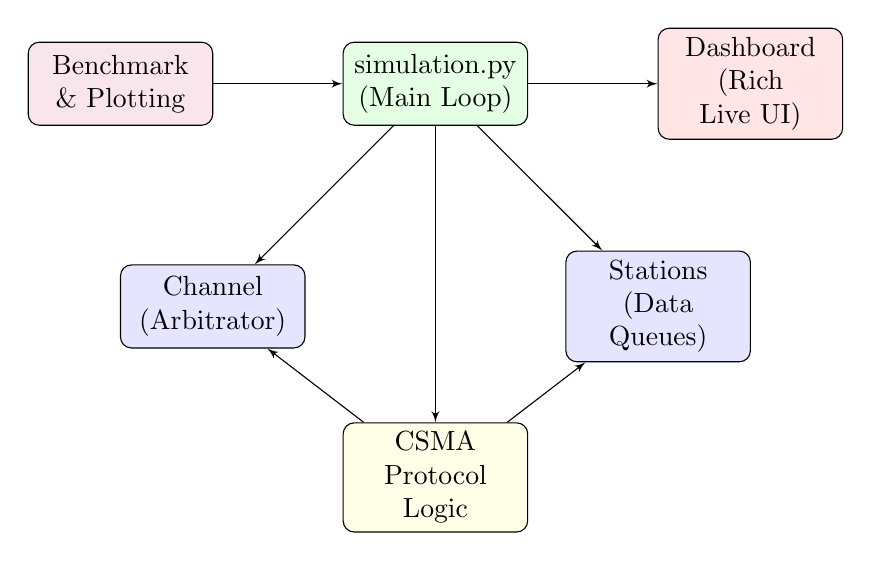
\begin{tikzpicture}[node distance=2cm, auto]
    \tikzstyle{block} = [rectangle, draw, fill=blue!10, text width=6em, text centered, rounded corners, minimum height=3em]
    \tikzstyle{line} = [draw, -latex']

    \node [block, fill=green!10] (main) {simulation.py (Main Loop)};
    \node [block, below left of=main, node distance=4cm] (channel) {Channel \\ (Arbitrator)};
    \node [block, below right of=main, node distance=4cm] (stations) {Stations \\ (Data Queues)};
    \node [block, below of=main, node distance=5cm, fill=yellow!10] (protocols) {CSMA \\ Protocol Logic};
    \node [block, right of=main, node distance=4cm, fill=red!10] (dashboard) {Dashboard \\ (Rich Live UI)};
    \node [block, left of=main, node distance=4cm, fill=purple!10] (benchmark) {Benchmark \\ \& Plotting};

    \path [line] (main) -- (channel);
    \path [line] (main) -- (stations);
    \path [line] (main) -- (protocols);
    \path [line] (main) -- (dashboard);
    \path [line] (benchmark) -- (main);
    \path [line] (protocols) -- (channel);
    \path [line] (protocols) -- (stations);
\end{tikzpicture}
\end{center}

\subsection{Input and Output Format}
\textbf{Input Format:} The simulator is driven via Command-Line Interfaces (CLI). Parameters like \texttt{--stations} ($N$), \texttt{--p-value}, \texttt{--sim-time}, and \texttt{--protocol} are passed at runtime. Additionally, a batch benchmarking script runs permutations without manual input.\\
\textbf{Output Format:} 
\begin{itemize}
    \item \textbf{Live Dashboard:} A \texttt{Rich}-based interactive terminal UI displaying real-time metrics and sparklines.
    \item \textbf{Tabular Summary:} Console output comparing Throughput, Utilization, and Collision Rates.
    \item \textbf{CSV \& Plots:} Automated generation of \texttt{results.csv} and 9 corresponding Matplotlib charts saved in the \texttt{plots/} directory.
\end{itemize}

\section{Implementation}

\subsection{Theory}
\textbf{Non-Persistent CSMA:} If the channel is busy, the station waits a random amount of time before sensing again.\\
\textbf{1-Persistent CSMA:} The station continuously senses the channel. Once idle, it transmits immediately with a probability of 1.\\
\textbf{p-Persistent CSMA:} The station continuously senses the channel. Once idle, it transmits with probability $p$. If it defers, it waits for the next slot.\\
\textbf{CSMA/CD (Collision Detection):} Follows 1-persistent logic, but nodes monitor the channel while transmitting. If a collision is detected, transmissions are immediately aborted, a jam signal is sent, and BEB is initiated.

\subsection{Code Snippets \& Interfaces}
The primary interface is the `Station` and `Channel` models, governed by a per-slot tick loop. Below are the implementation snippets for the four \textbf{CSMA} protocol variants, evaluating state per-slot:

\begin{lstlisting}[language=Python, caption=Non-Persistent CSMA]
def non_persistent_csma(station: Station, channel: Channel, current_time: float, slot_time: float) -> bool:
    if channel.sense(current_time) == ChannelState.IDLE:
        return True # Transmit
    else:
        wait_slots = random.randint(1, 10)
        station.set_deferred(wait_slots * slot_time)
        return False
\end{lstlisting}

\begin{lstlisting}[language=Python, caption=1-Persistent CSMA]
def one_persistent_csma(station: Station, channel: Channel, current_time: float) -> bool:
    if channel.sense(current_time) == ChannelState.IDLE:
        return True
    return False # Busy-wait: keep sensing
\end{lstlisting}

\begin{lstlisting}[language=Python, caption=p-Persistent CSMA]
def p_persistent_csma(station: Station, channel: Channel, current_time: float, slot_time: float, p: float = 0.3) -> bool:
    if channel.sense(current_time) == ChannelState.IDLE:
        if random.random() < p:
            return True
        else:
            station.set_deferred(slot_time)
    return False
\end{lstlisting}

\begin{lstlisting}[language=Python, caption=CSMA/CD Protocol Logic]
def csma_cd(station: Station, channel: Channel, current_time: float) -> bool:
    # 1-persistent sense, actual abort logic is handled in the main loop
    if channel.sense(current_time) == ChannelState.IDLE:
        return True
    return False
\end{lstlisting}

\begin{lstlisting}[language=Python, caption=Collision Detection in Main Loop]
# Apply all simultaneous transmission attempts
for sid in want_to_transmit:
    channel.attempt_transmission(sid, current_time, config.frame_duration)

# Check for collisions (2+ stations transmitted this slot)
if channel.check_collision():
    collided_ids = channel.abort_all_transmissions(current_time)
    if protocol_name == "csma_cd":
        channel.send_jam_signal(current_time, config.jam_duration)
    for sid in collided_ids:
        stations[sid].handle_collision(current_time, config.slot_time)
\end{lstlisting}

\section{Test Cases}

The simulation was thoroughly verified using both unit-level logging and high-level metric validation.

\begin{table}[h]
\centering
\begin{tabular}{@{}p{3cm} p{5cm} p{6cm}@{}}
\toprule
\textbf{Test Case} & \textbf{Sample Test Data} & \textbf{What is Checked} \\
\midrule
\textbf{TC1: Channel Collision Arbitrator} & N=2, both TX at t=0, Propagation Delay = 2 slots. & Ensures \texttt{check\_collision()} triggers when $N \ge 2$ overlap within vulnerability window, and \texttt{abort\_all\_transmissions()} clears state. \\
\textbf{TC2: p-Persistent Probability} & N=1, p=0.1, 1000 slots. & Ensures the isolated station defers $\sim 90\%$ of the time when channel is idle, resulting in higher latency but no collisions. \\
\textbf{TC3: Load Saturation} & N=30, 1-Persistent, 5000 slots. & Checks network saturation behavior. Expects 1-Persistent throughput to plummet toward zero as continuous collisions cause BEB lock-out. \\
\textbf{TC4: Live Dashboard State} & \texttt{--protocol all --dashboard} & Ensures dashboard correctly tracks UI states across 4 consecutive simulations without dropping threads or zeroing metrics. \\
\bottomrule
\end{tabular}
\caption{Designed Test Cases}
\end{table}

\section{Results}

Extensive benchmarking was performed by sweeping $N \in [2, 30]$ and $p \in [0.1, 0.9]$. The evaluation metrics included \textbf{Throughput} (successful frames per slot), \textbf{Average Delay} (wait time per frame), and \textbf{Collision Count}.

\begin{figure}[h]
    \centering
    \begin{minipage}{0.48\textwidth}
        \centering
        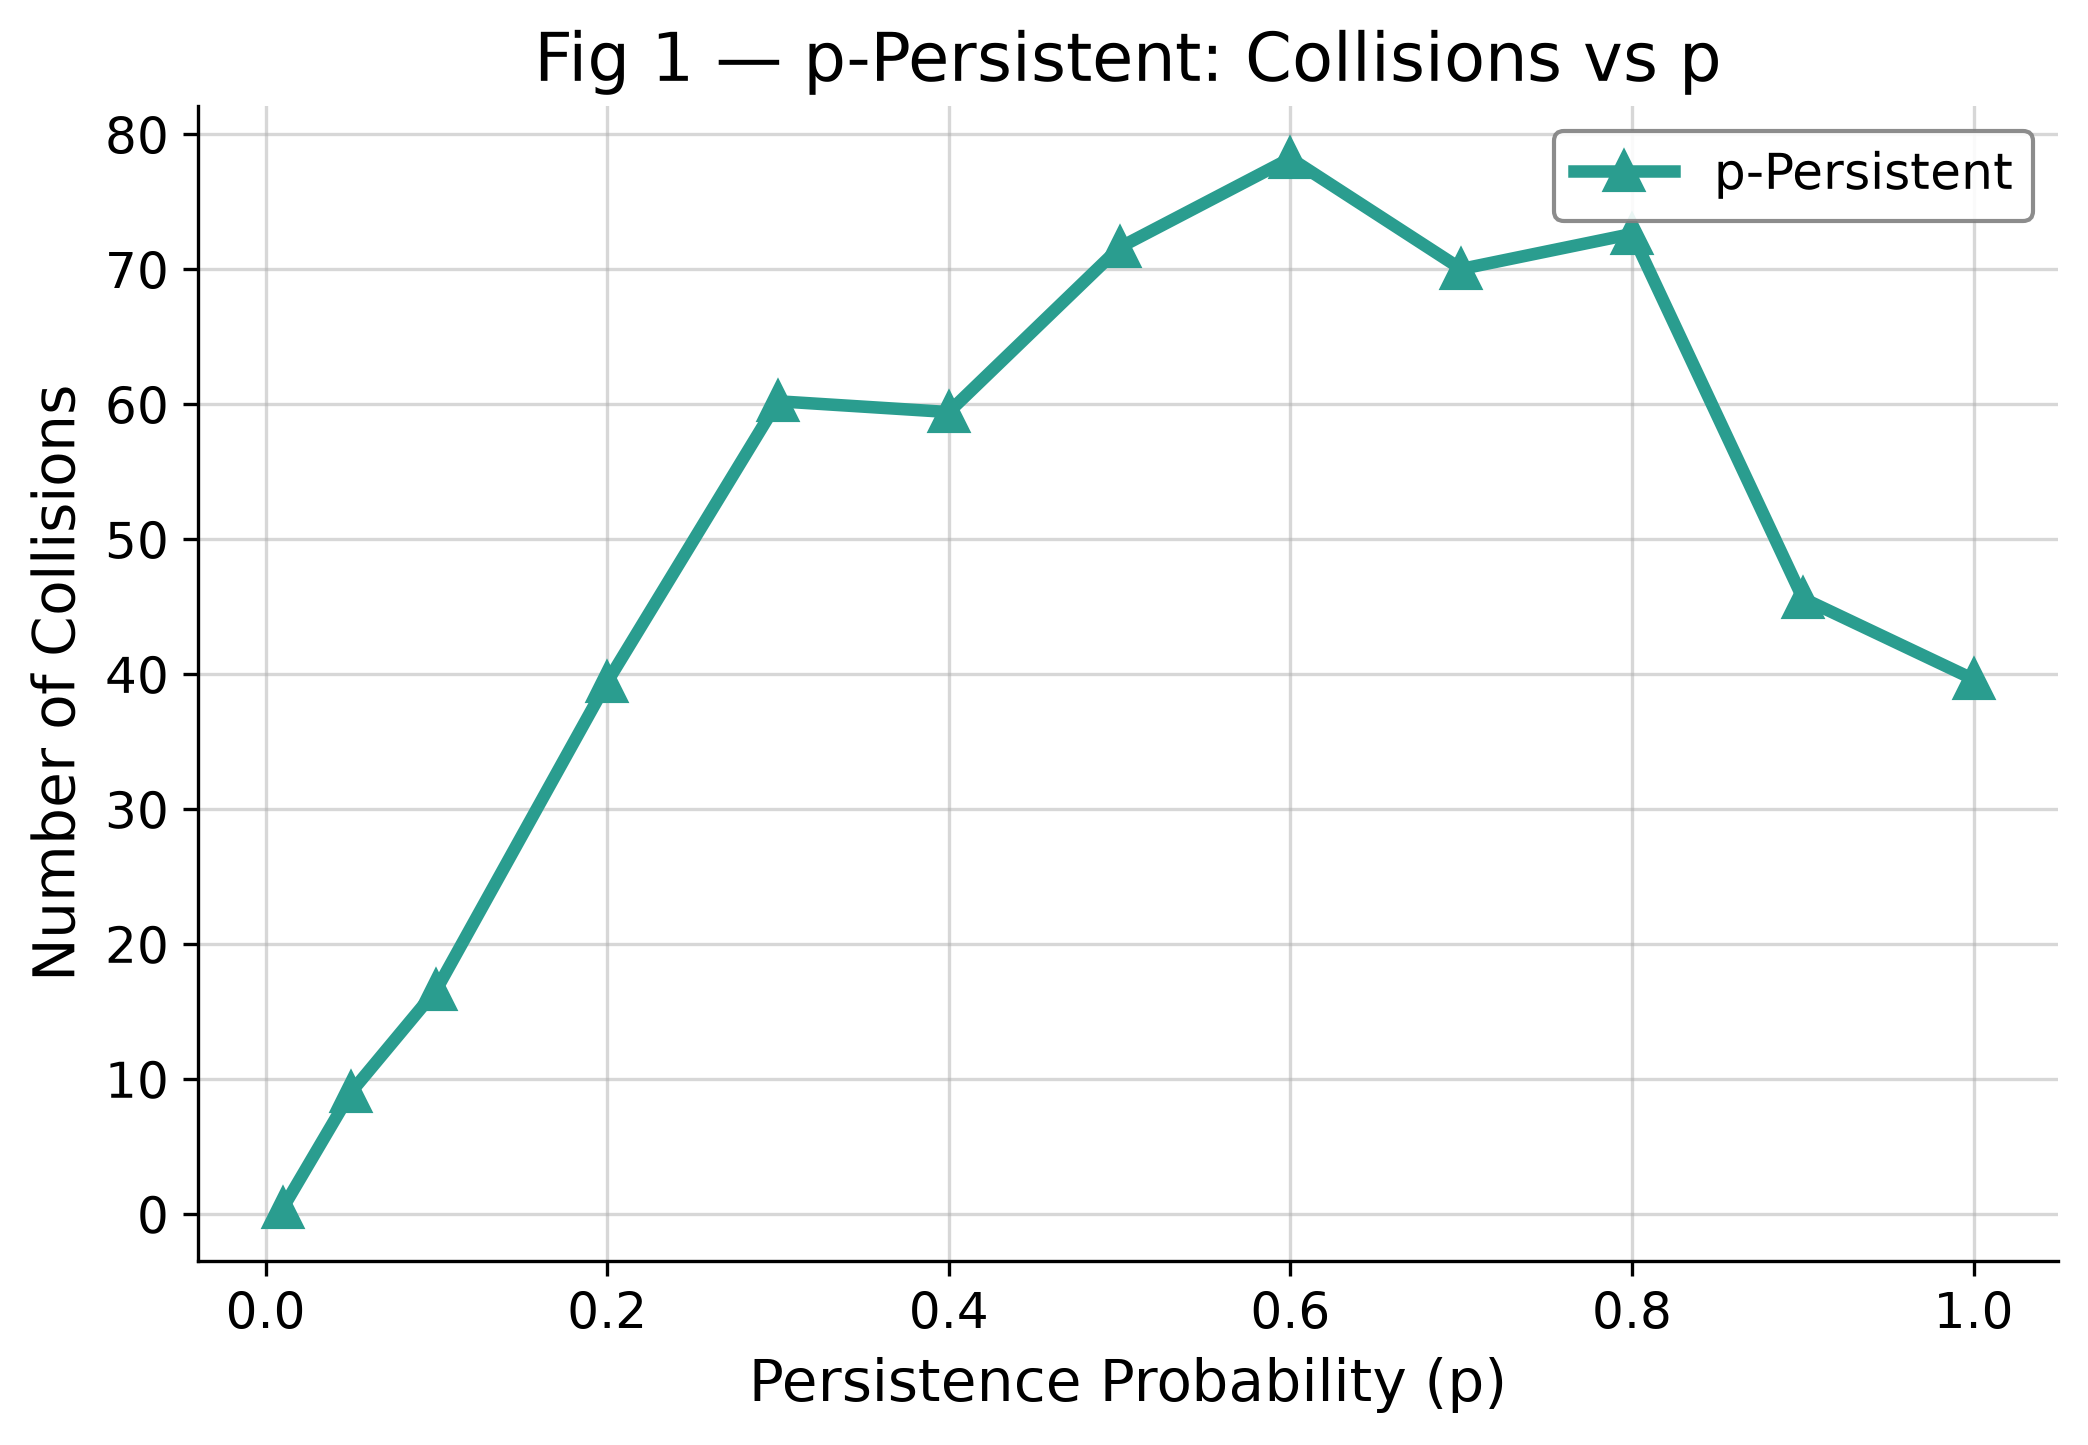
\includegraphics[width=\textwidth]{plots/fig1_p_collisions.png}
        \caption{Collisions vs Probability (p)}
    \end{minipage}\hfill
    \begin{minipage}{0.48\textwidth}
        \centering
        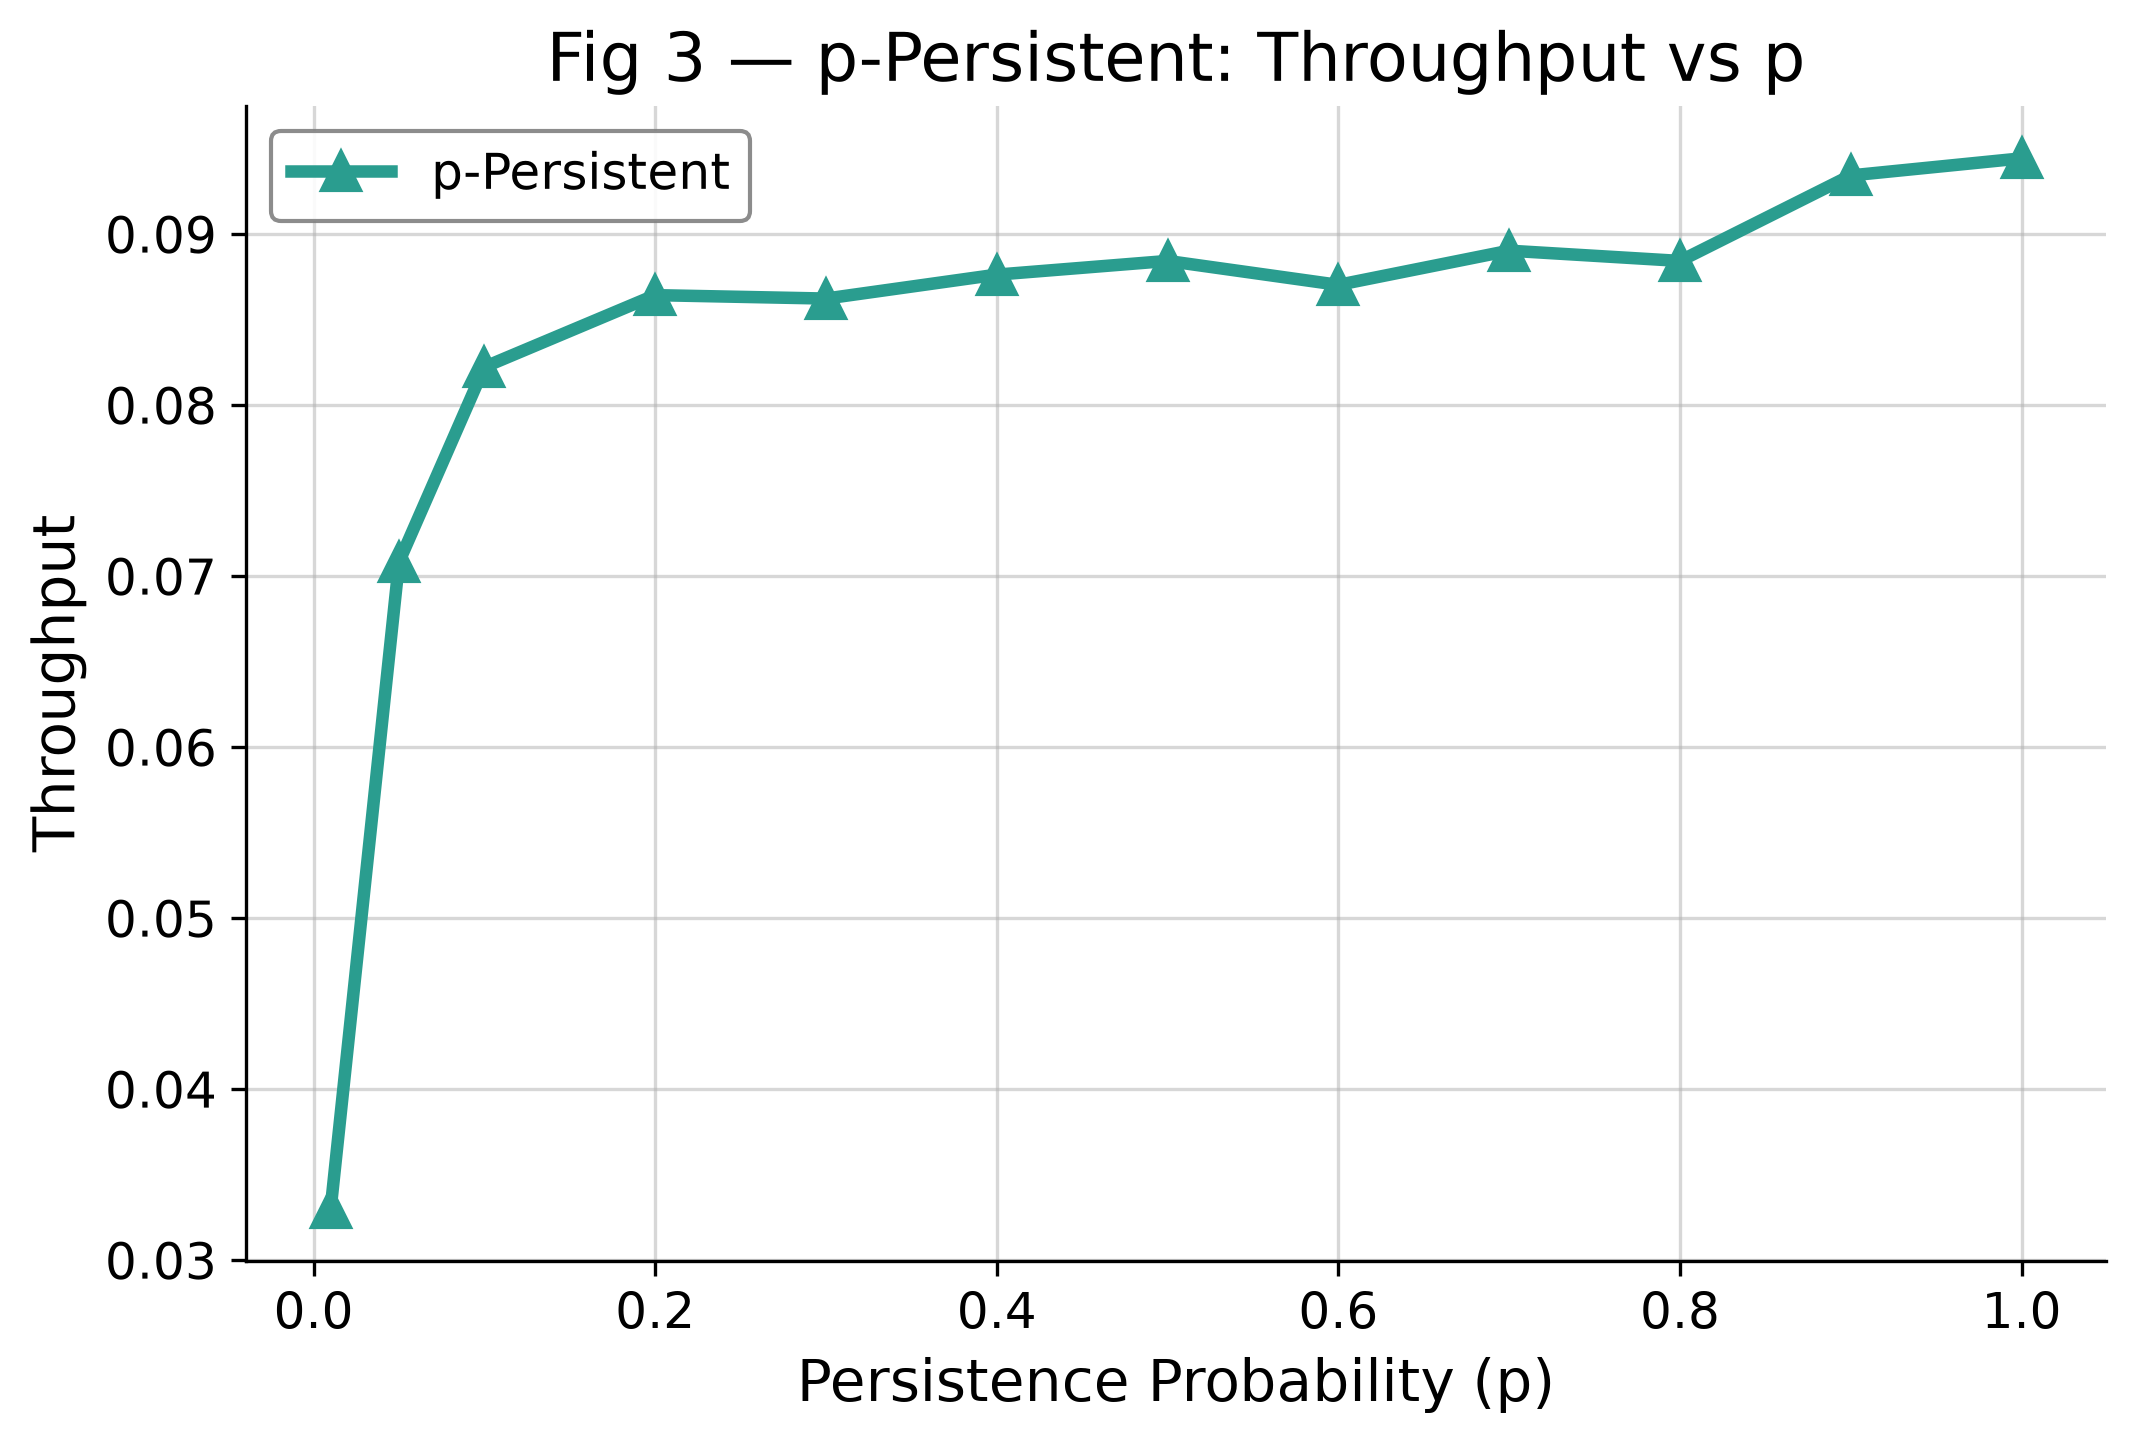
\includegraphics[width=\textwidth]{plots/fig3_p_throughput.png}
        \caption{Throughput vs Probability (p)}
    \end{minipage}
\end{figure}

\begin{figure}[h]
    \centering
    \begin{minipage}{0.48\textwidth}
        \centering
        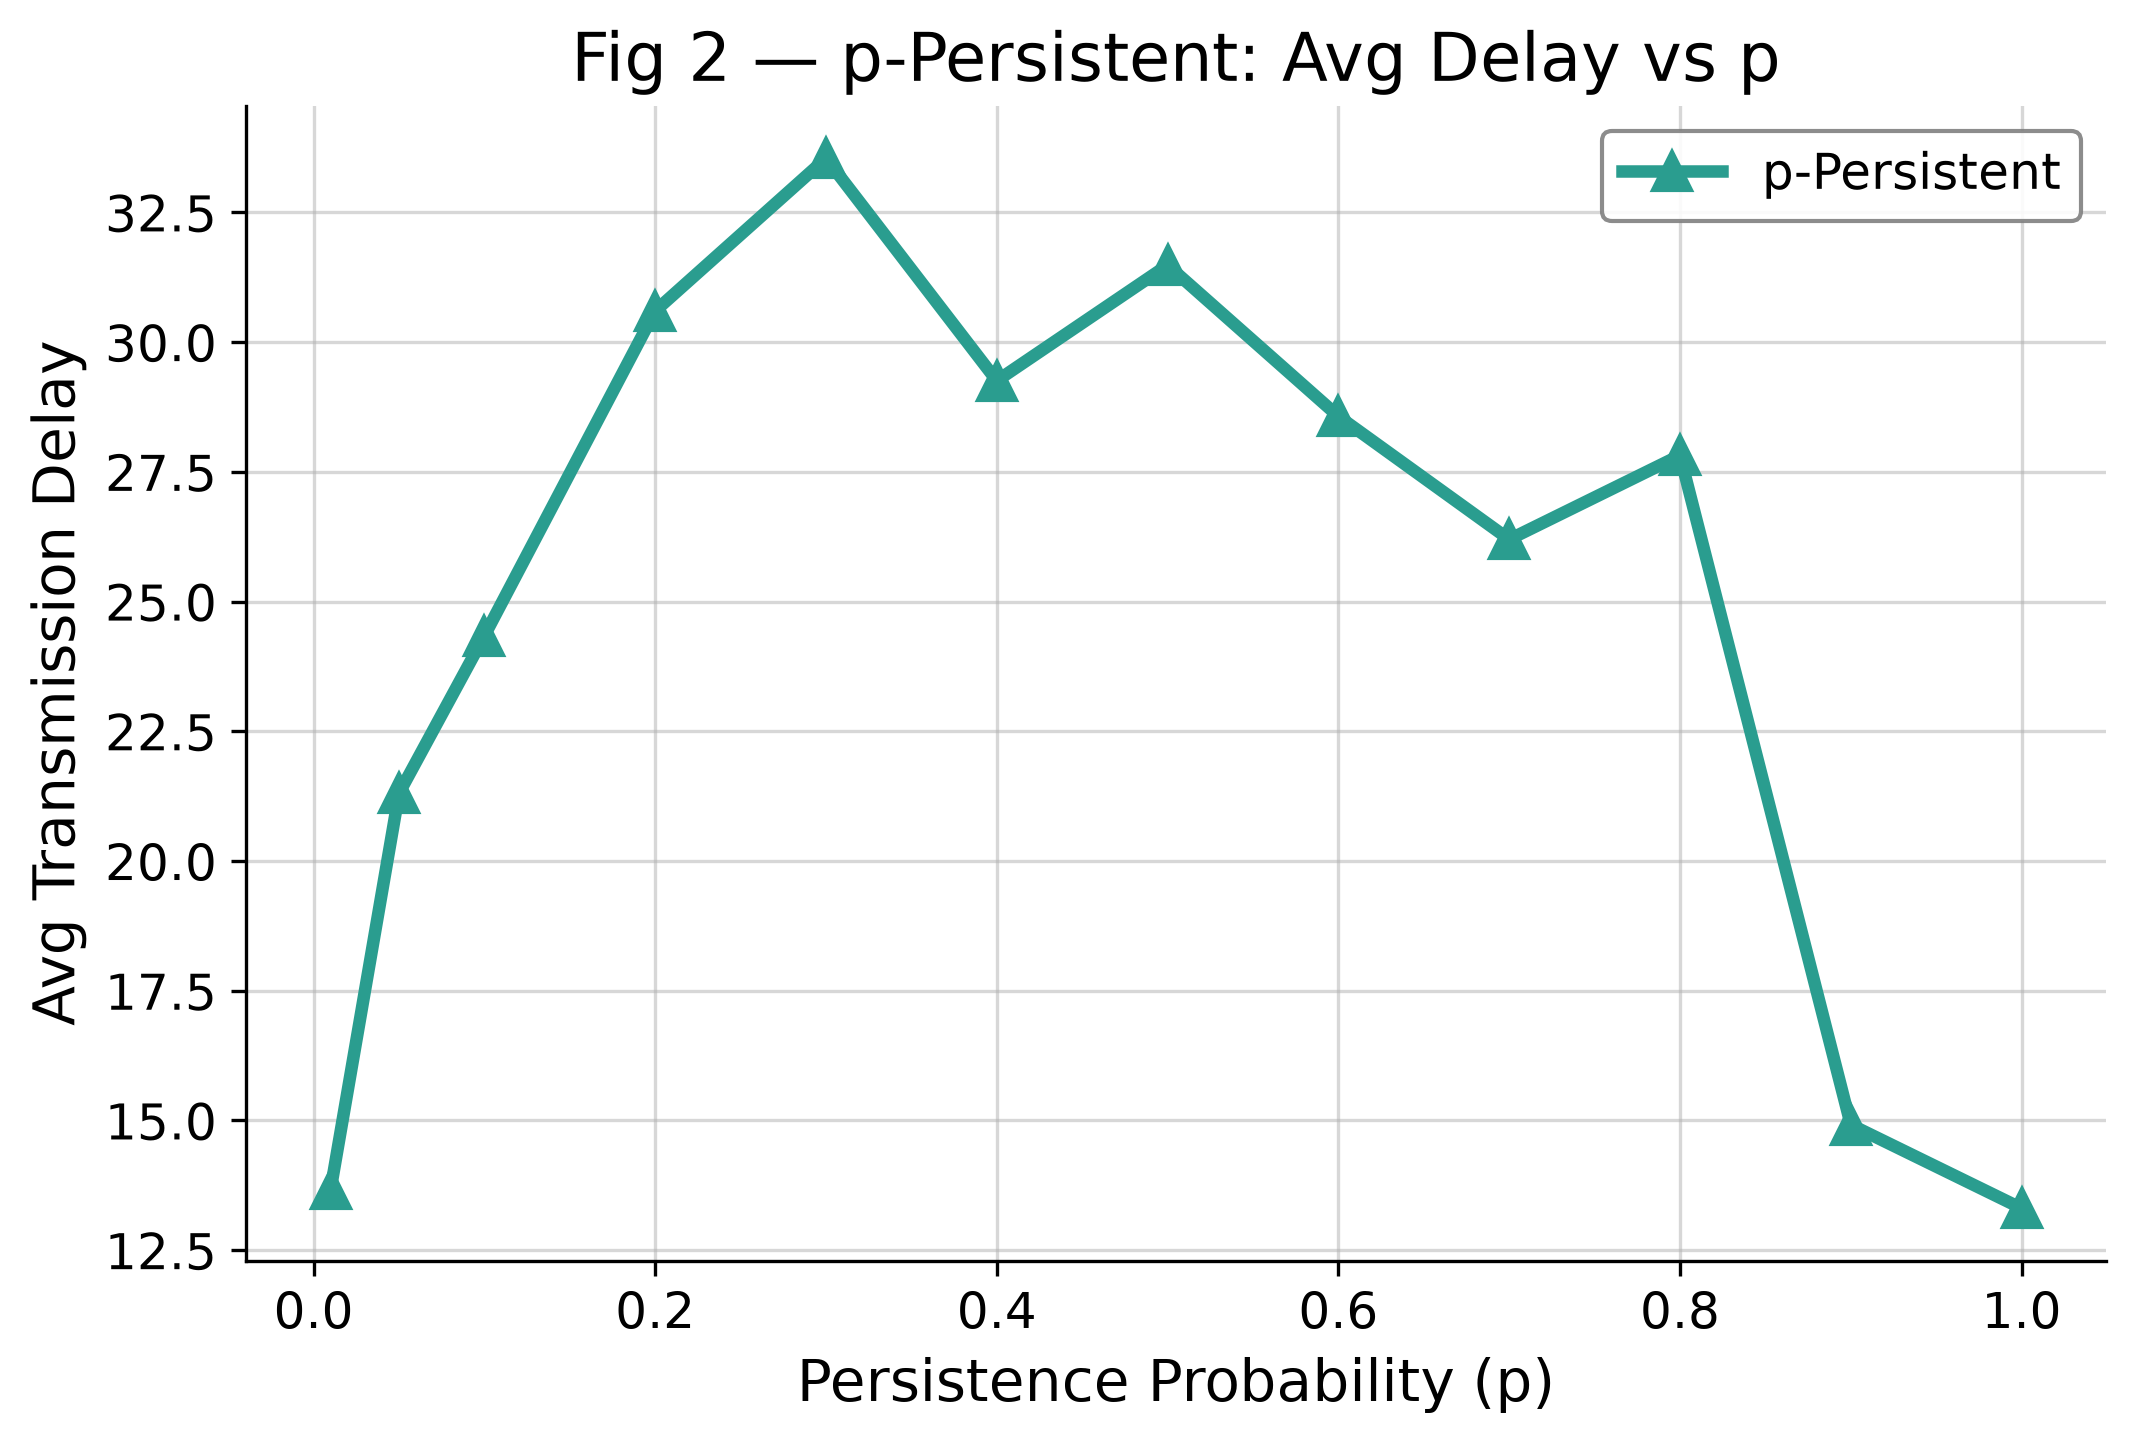
\includegraphics[width=\textwidth]{plots/fig2_p_delay.png}
        \caption{Delay vs Probability (p)}
    \end{minipage}\hfill
    \begin{minipage}{0.48\textwidth}
        \centering
        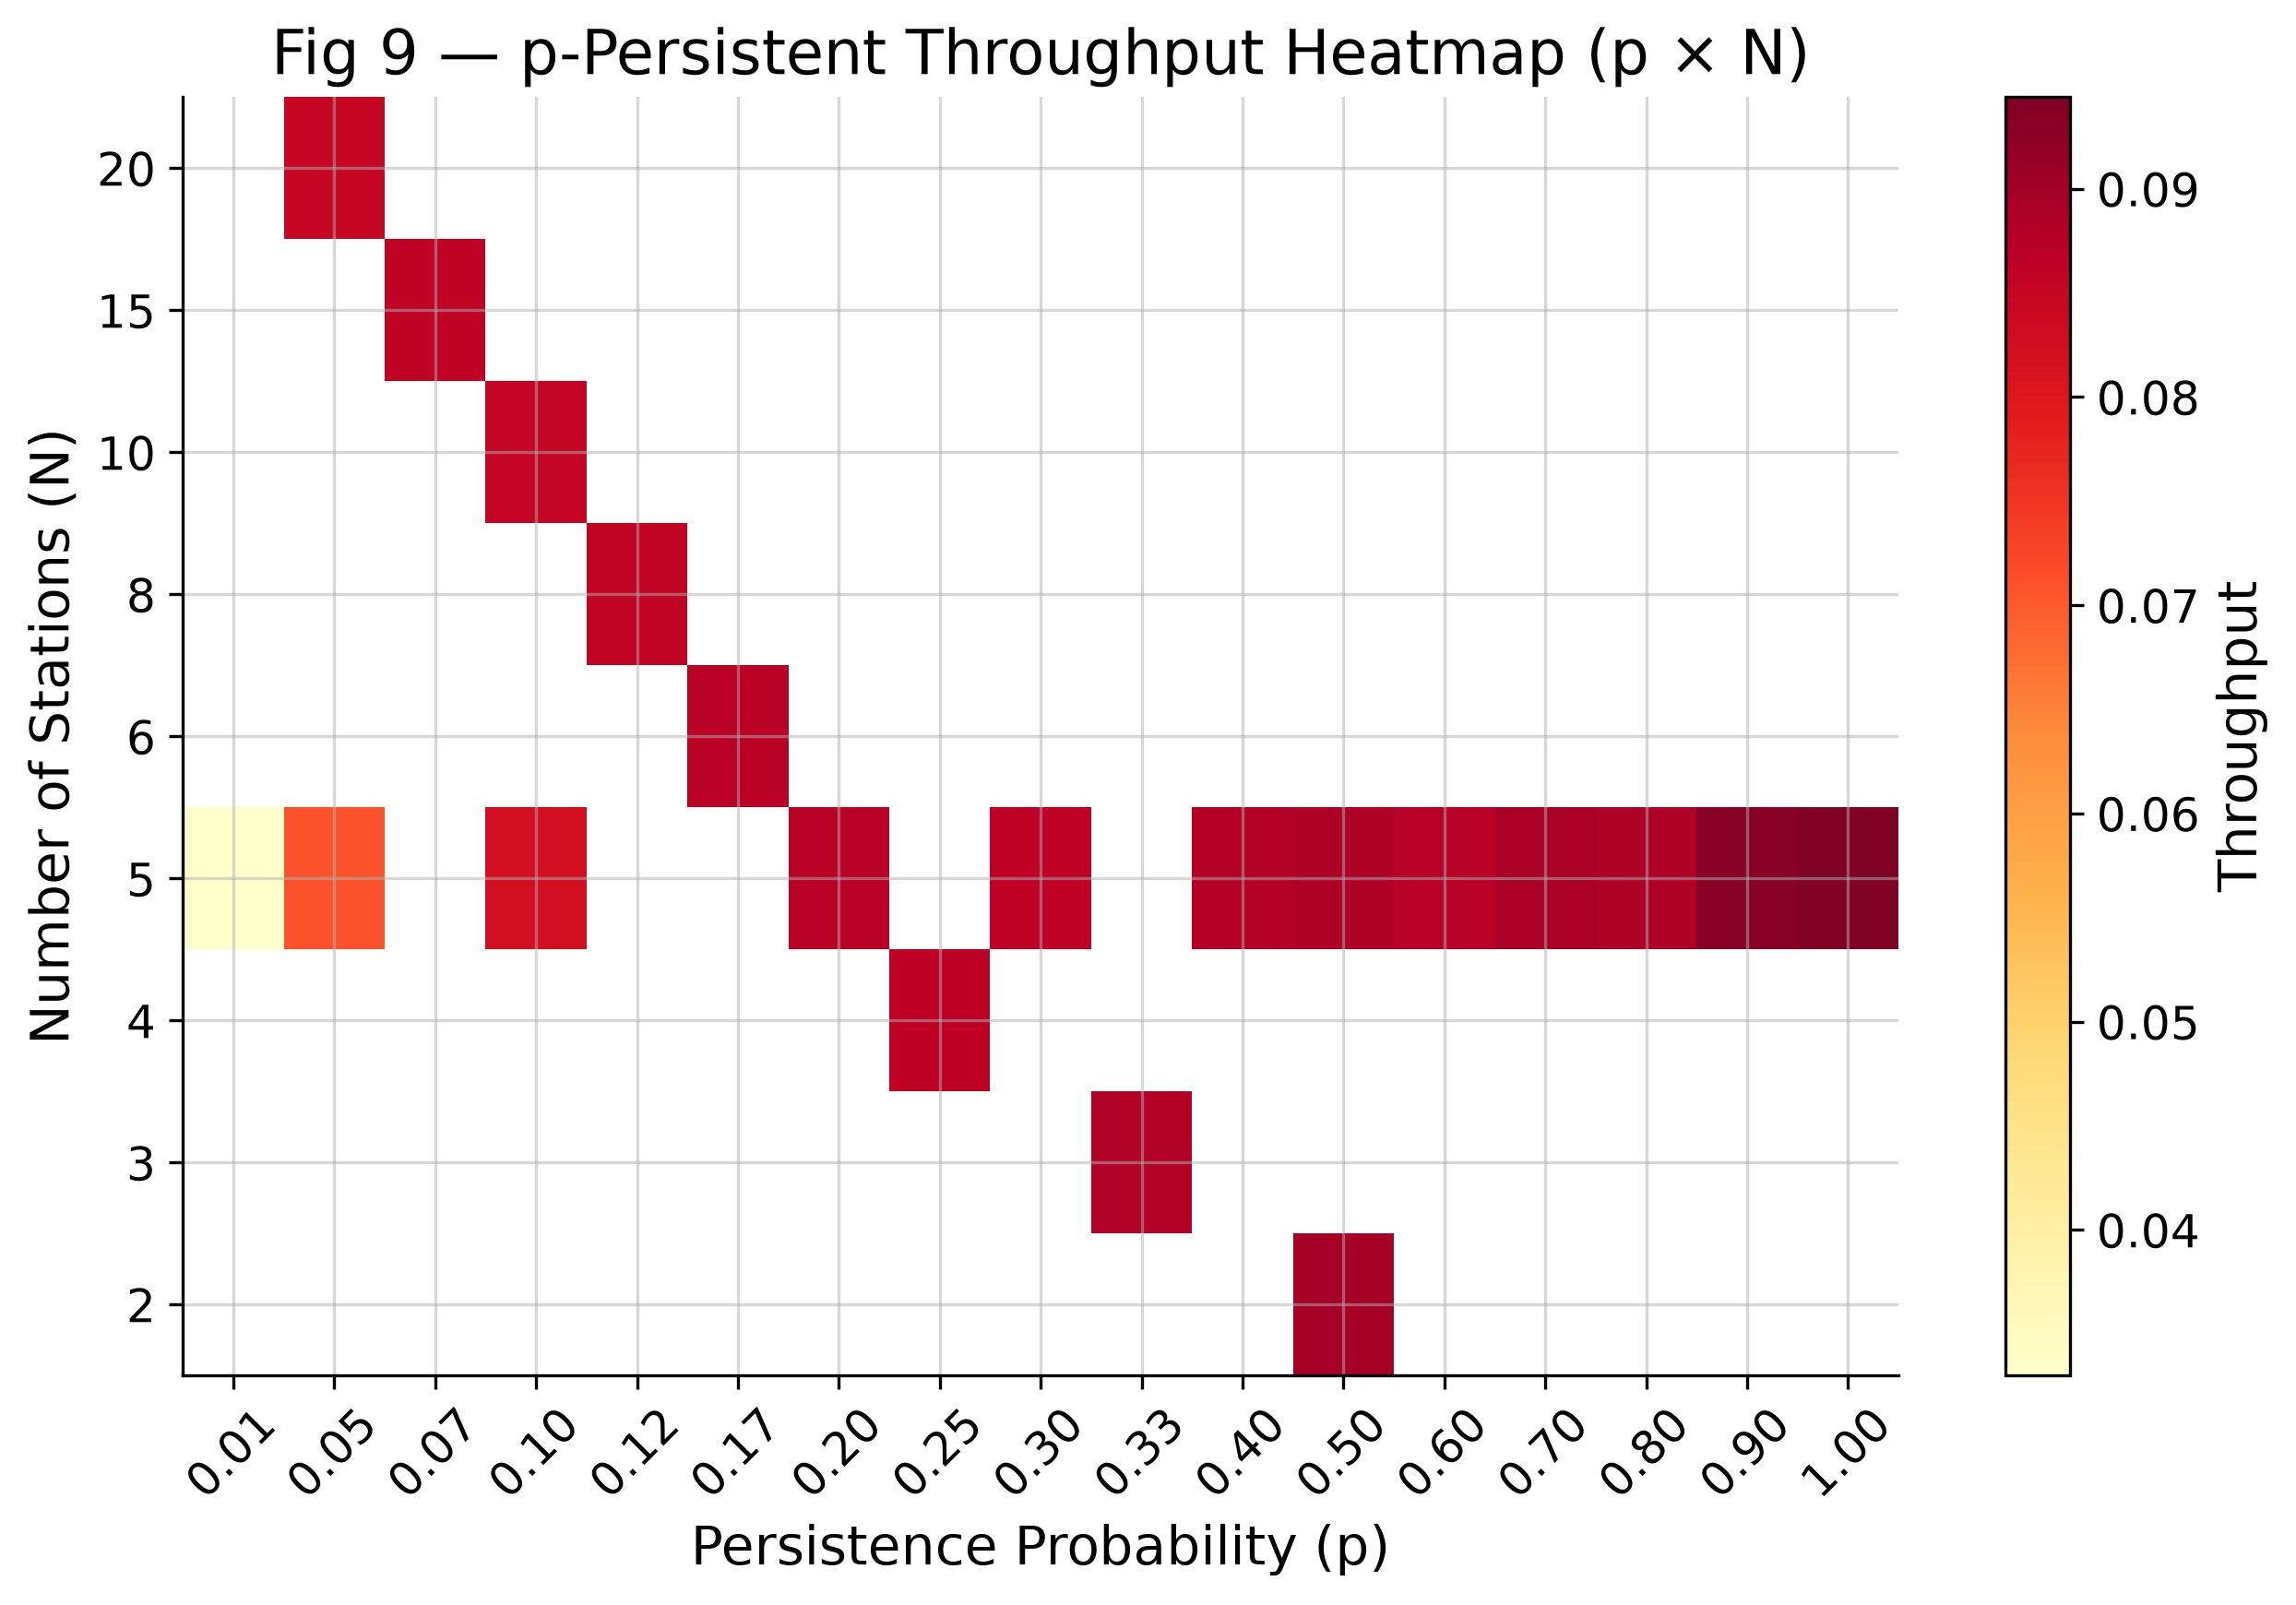
\includegraphics[width=\textwidth]{plots/fig9_p_heatmap.png}
        \caption{p-Persistent Heatmap}
    \end{minipage}
\end{figure}

\begin{figure}[h]
    \centering
    \begin{minipage}{0.48\textwidth}
        \centering
        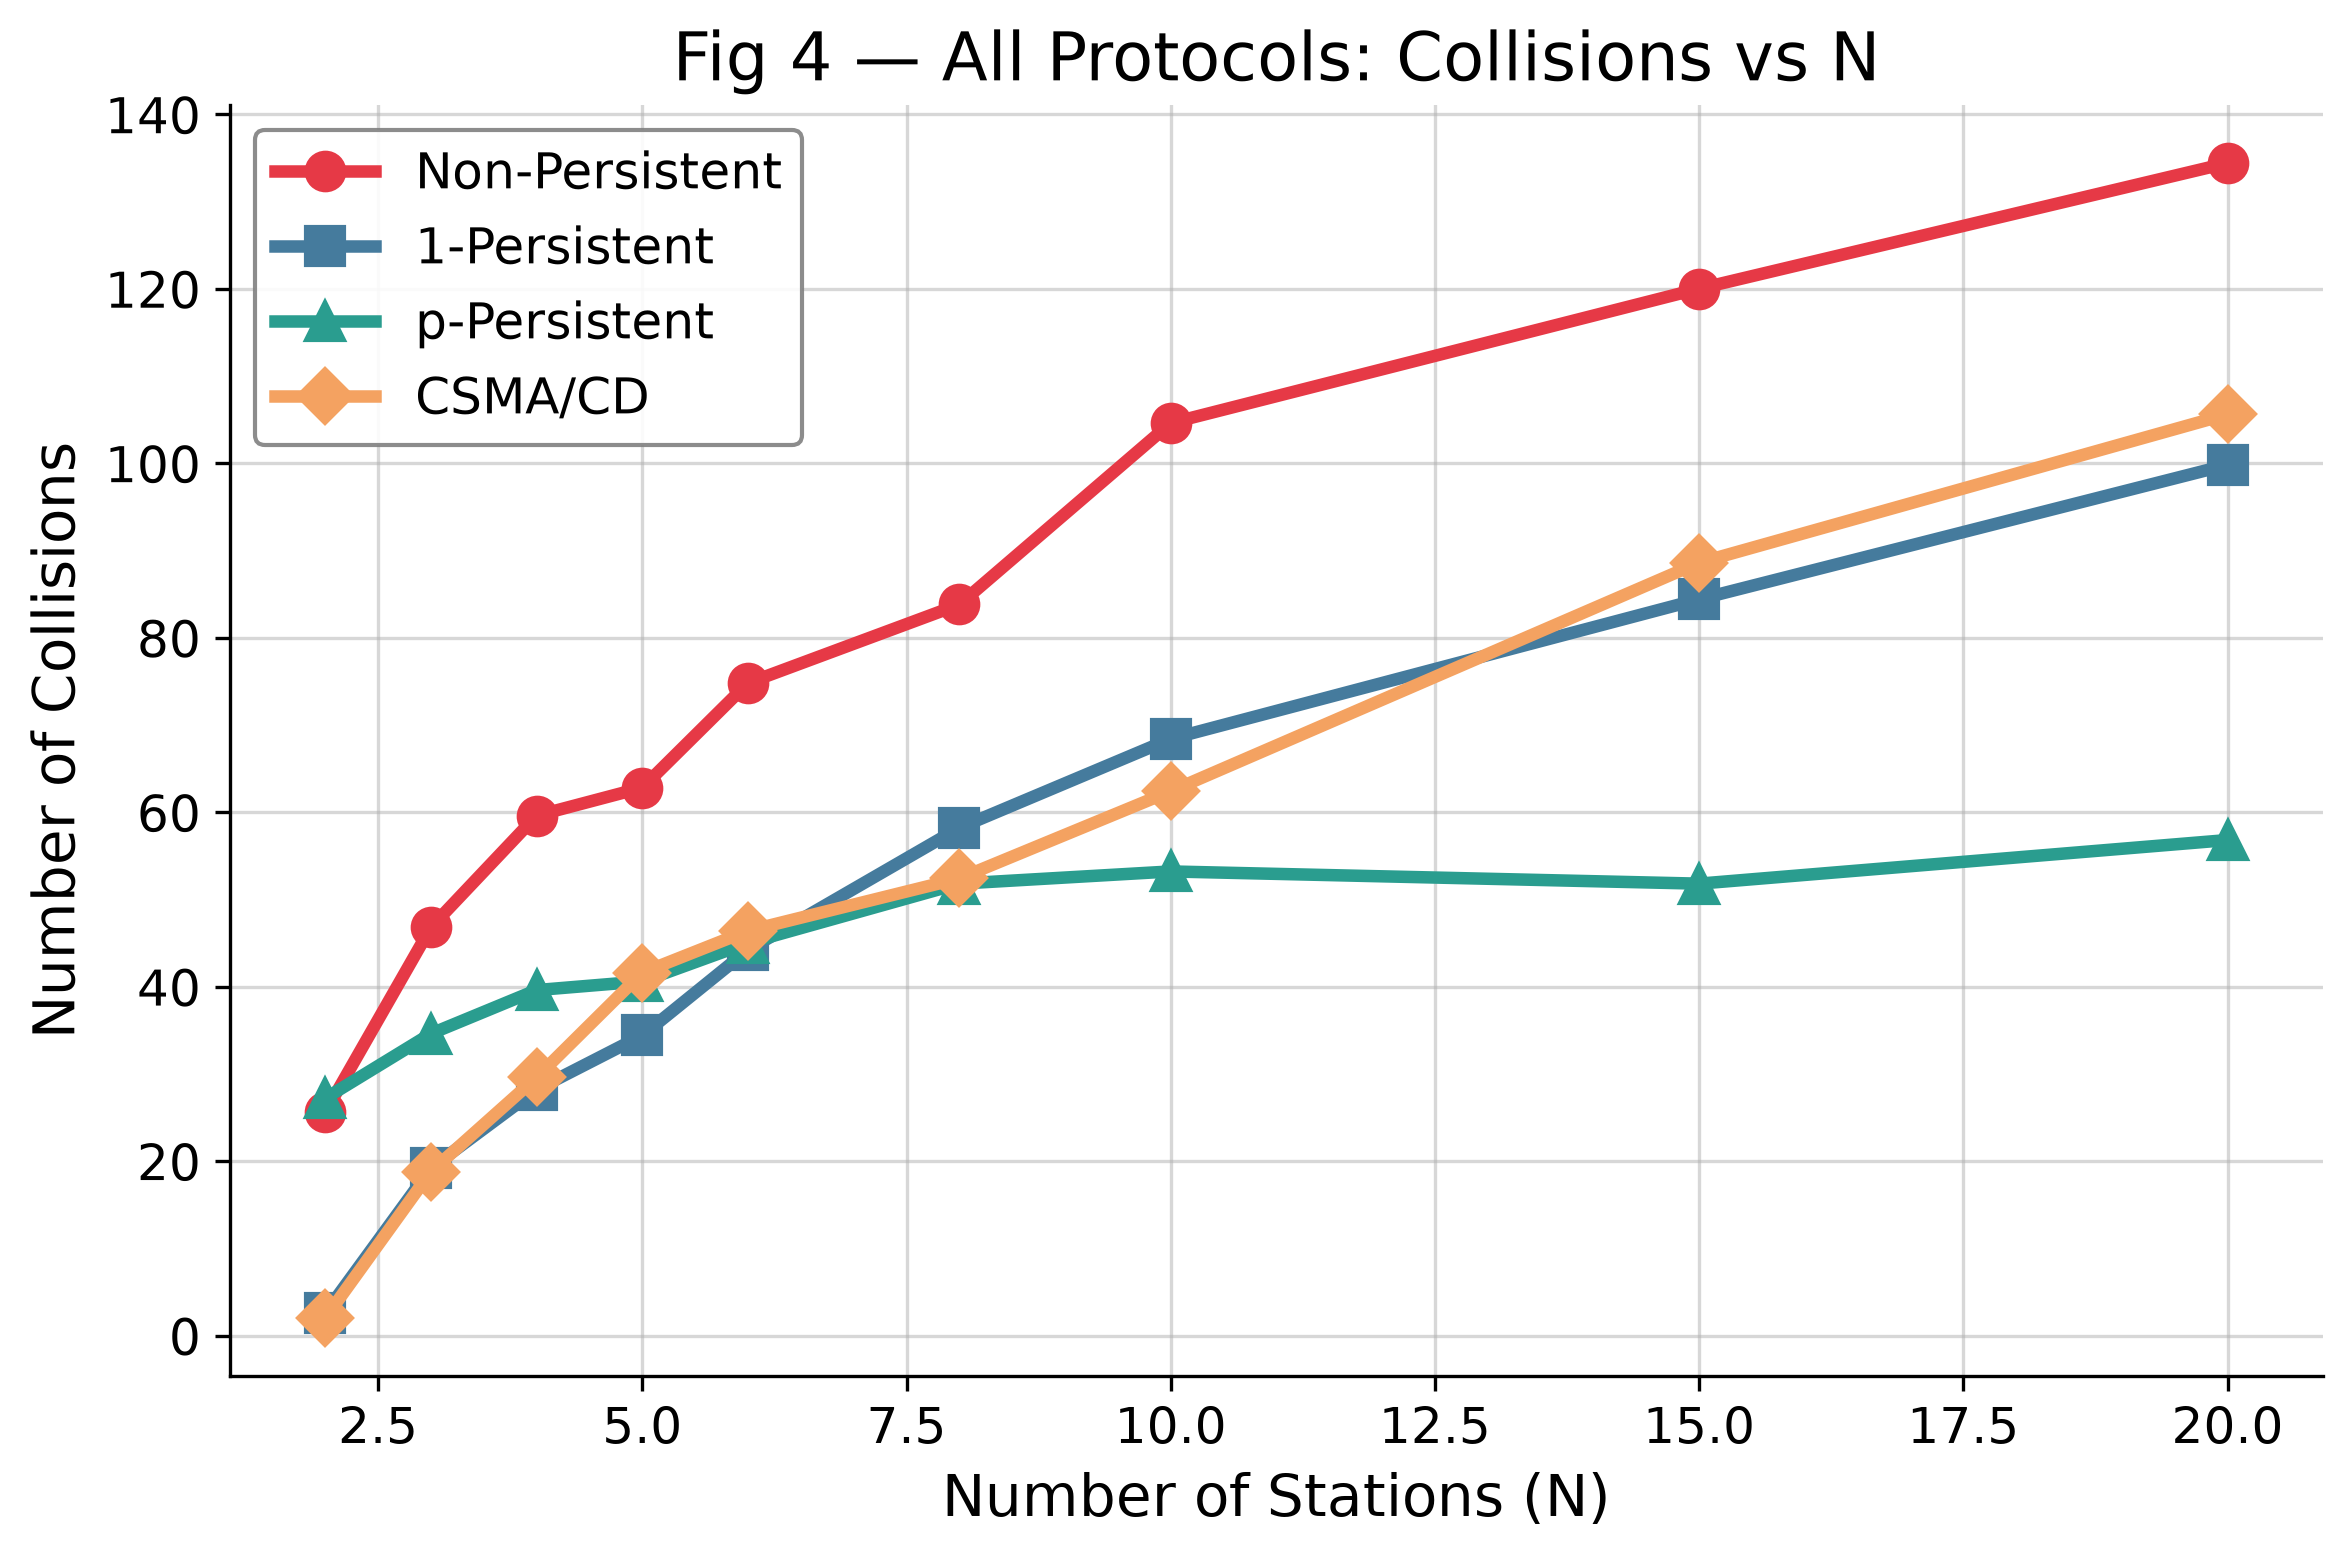
\includegraphics[width=\textwidth]{plots/fig4_n_collisions.png}
        \caption{Collisions vs Stations (N)}
    \end{minipage}\hfill
    \begin{minipage}{0.48\textwidth}
        \centering
        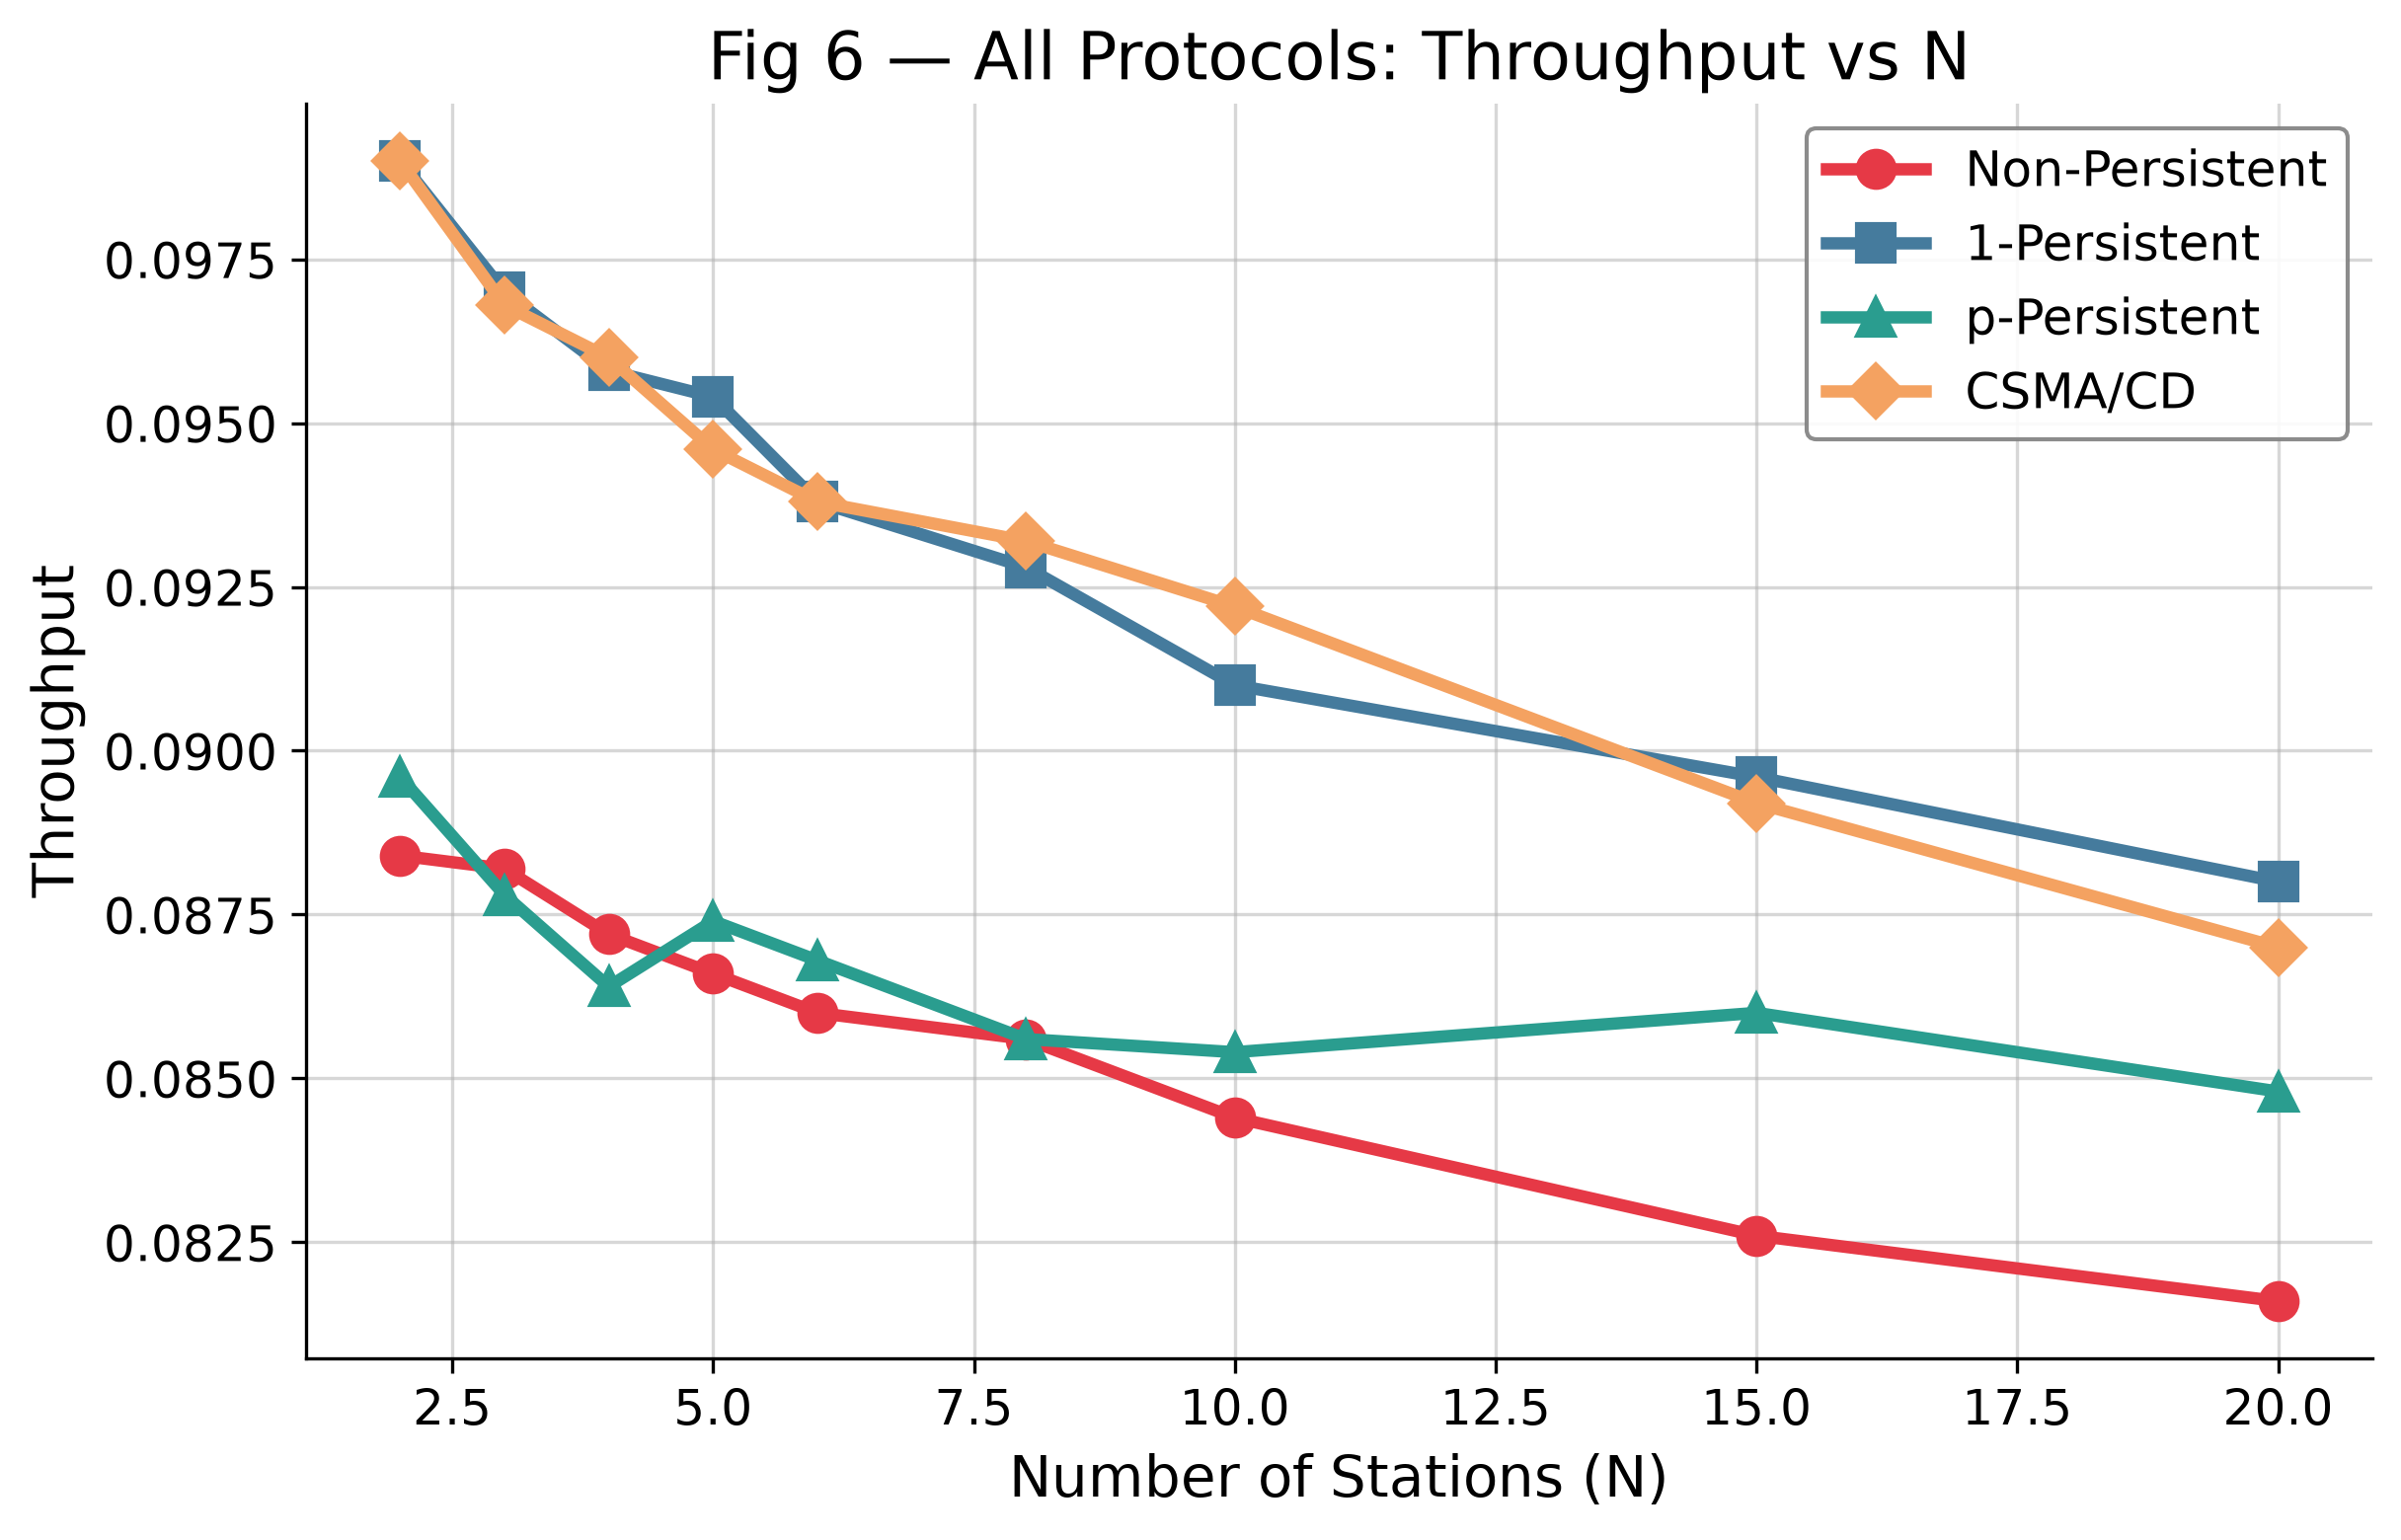
\includegraphics[width=\textwidth]{plots/fig6_n_throughput.png}
        \caption{Throughput vs Stations (N)}
    \end{minipage}
\end{figure}

\begin{figure}[h]
    \centering
    \begin{minipage}{0.48\textwidth}
        \centering
        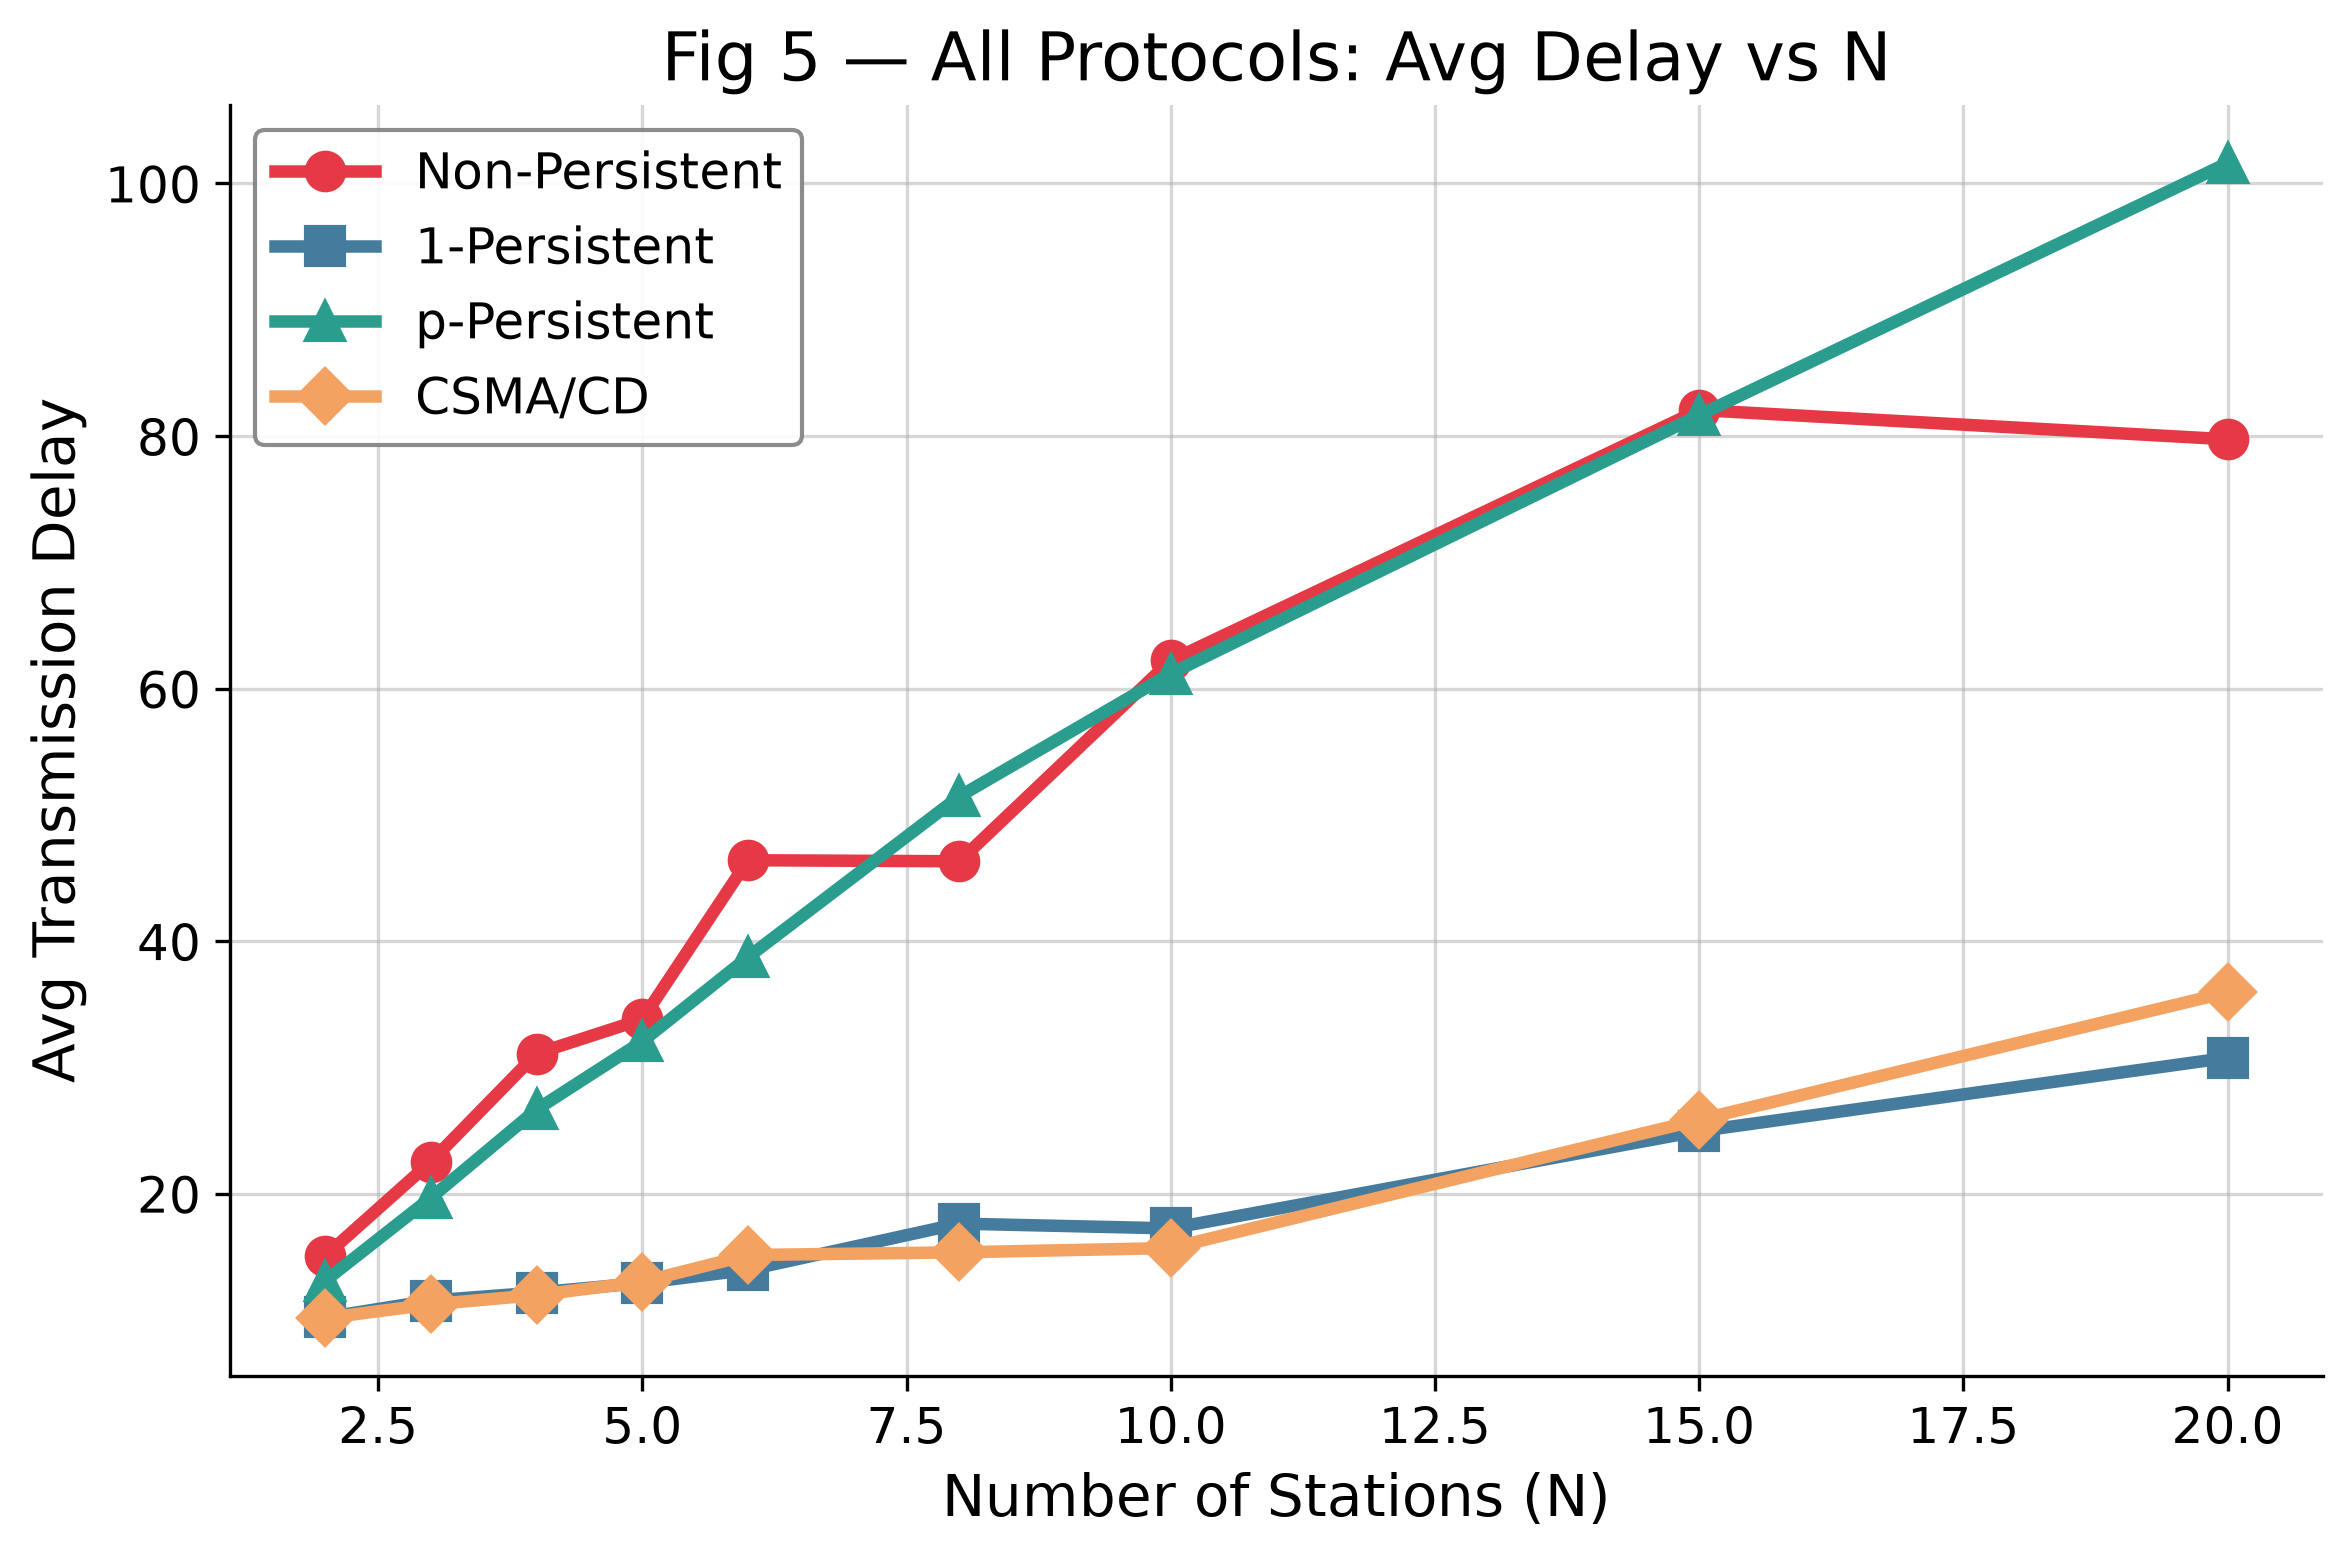
\includegraphics[width=\textwidth]{plots/fig5_n_delay.png}
        \caption{Delay vs Stations (N)}
    \end{minipage}\hfill
    \begin{minipage}{0.48\textwidth}
        \centering
        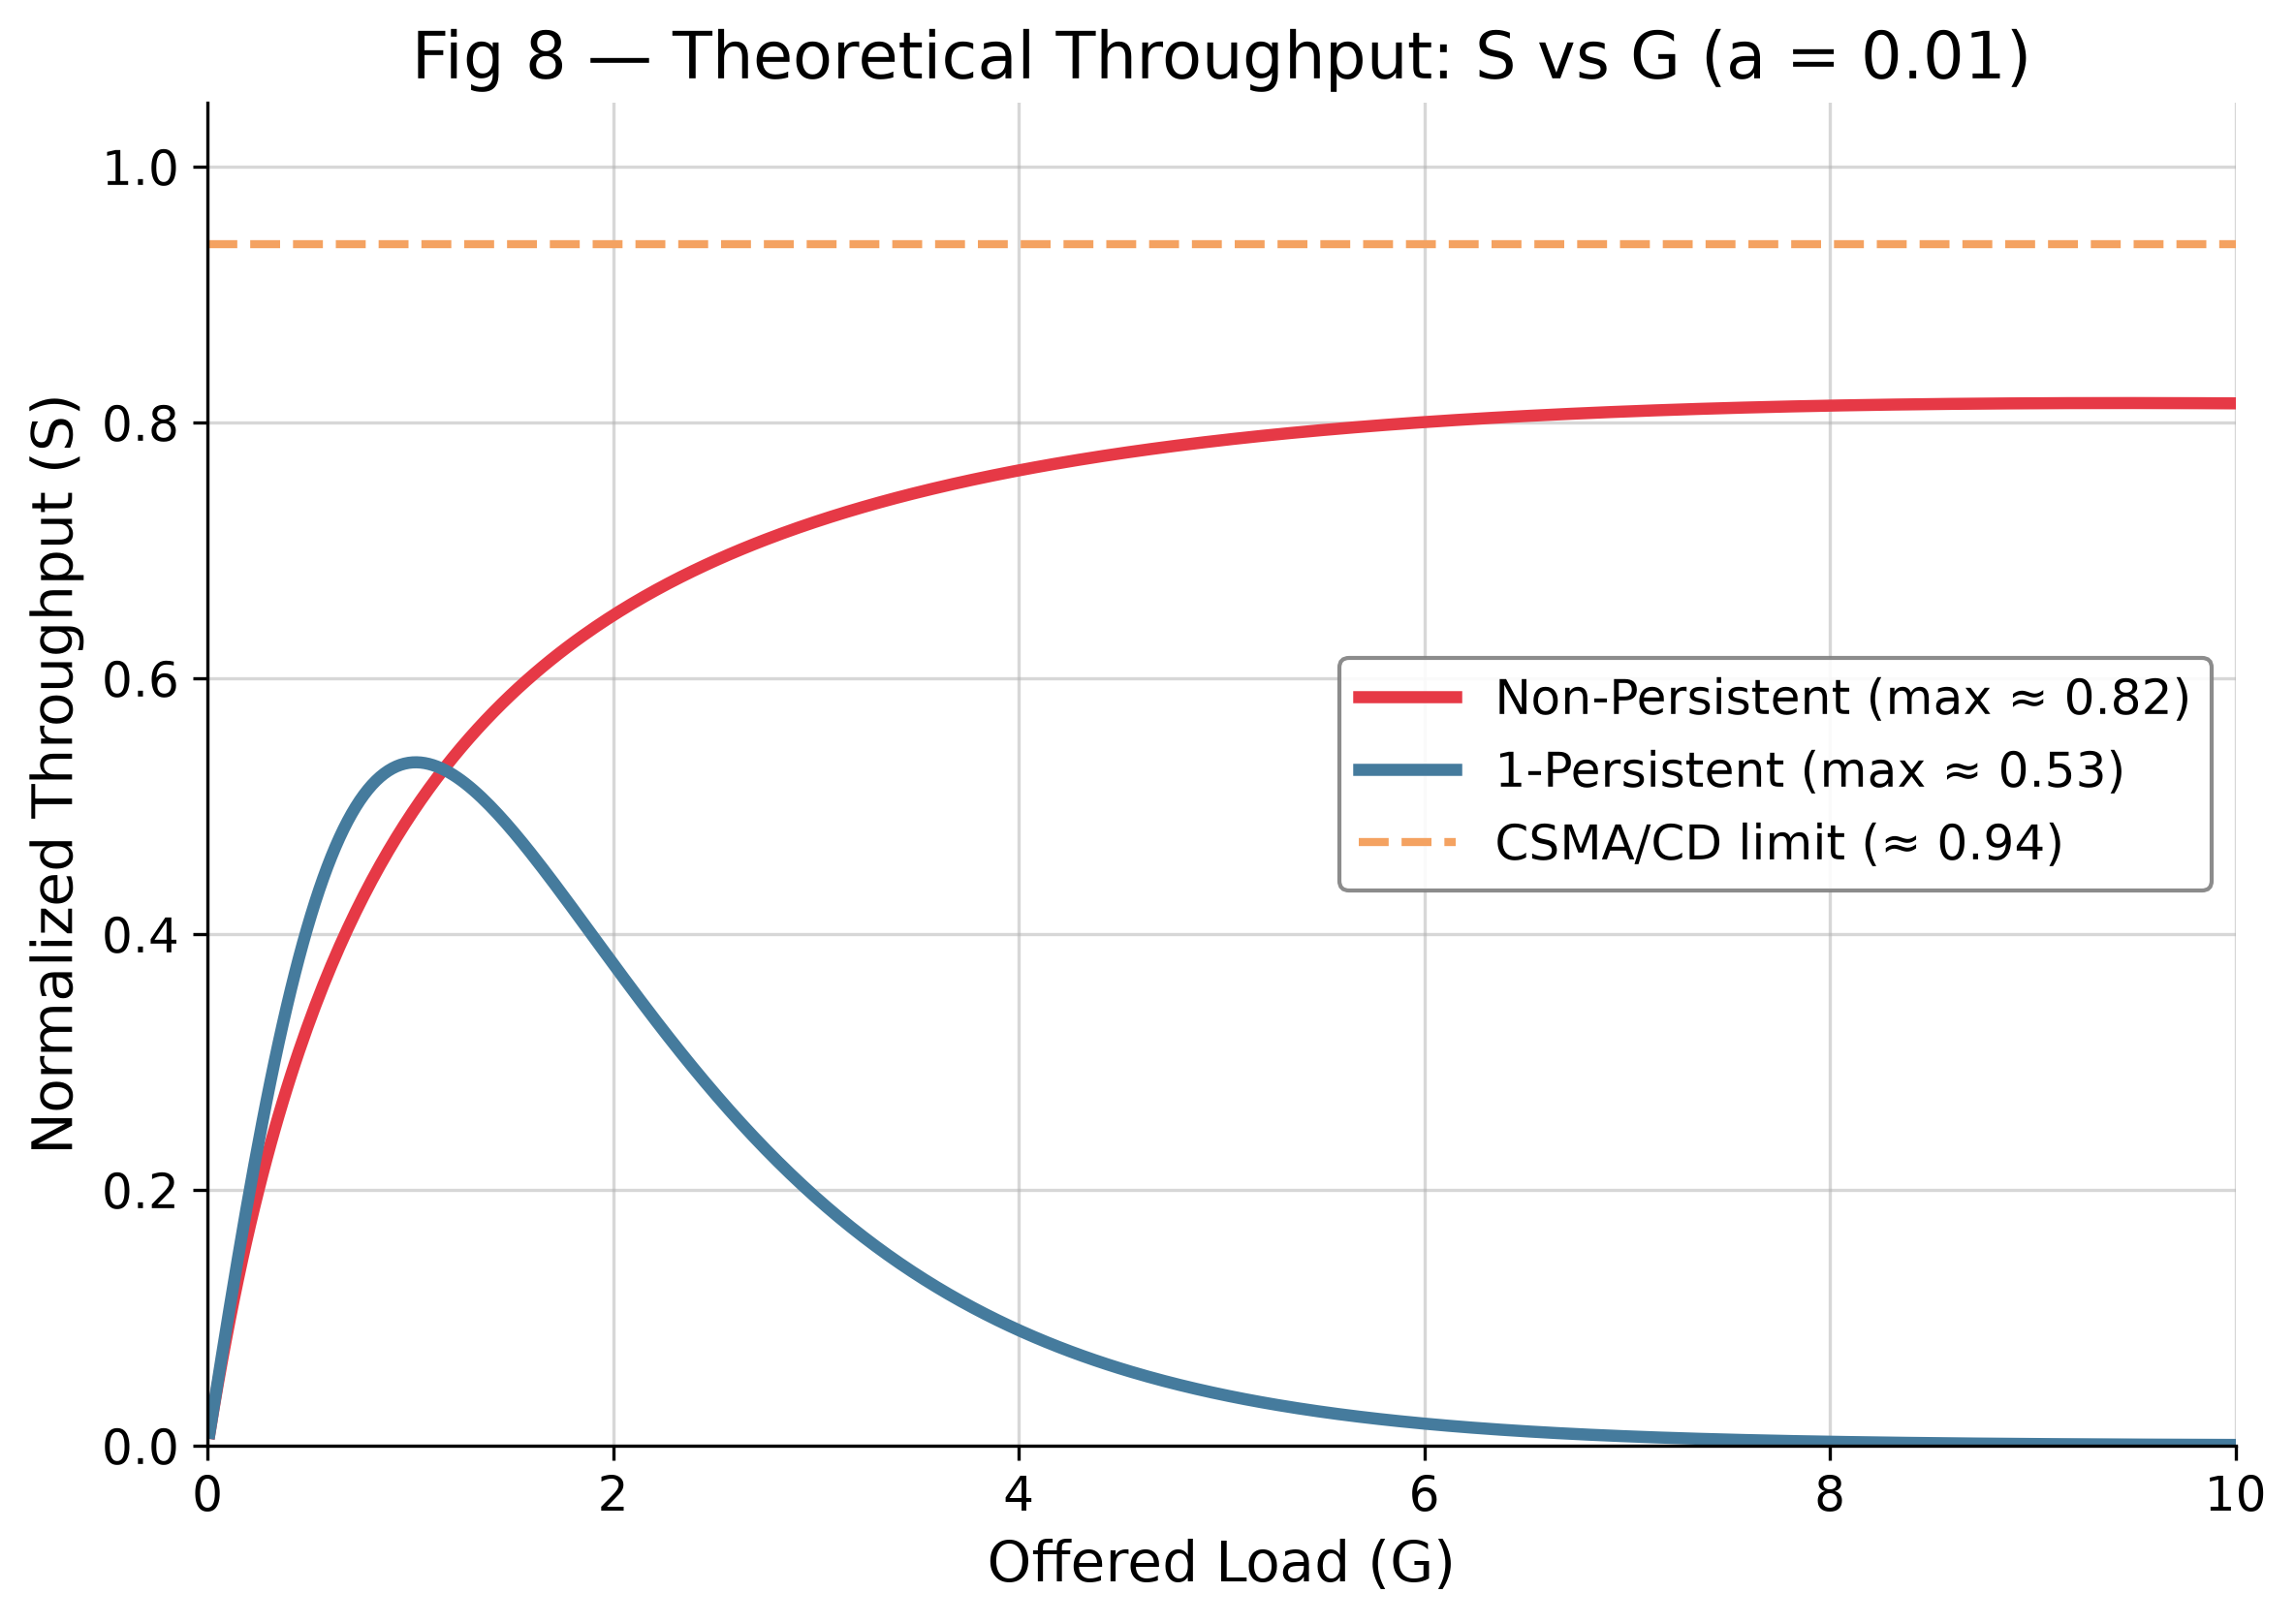
\includegraphics[width=\textwidth]{plots/fig8_theoretical_throughput.png}
        \caption{Theoretical Throughput Comparison}
    \end{minipage}
\end{figure}

\begin{figure}[h]
    \centering
    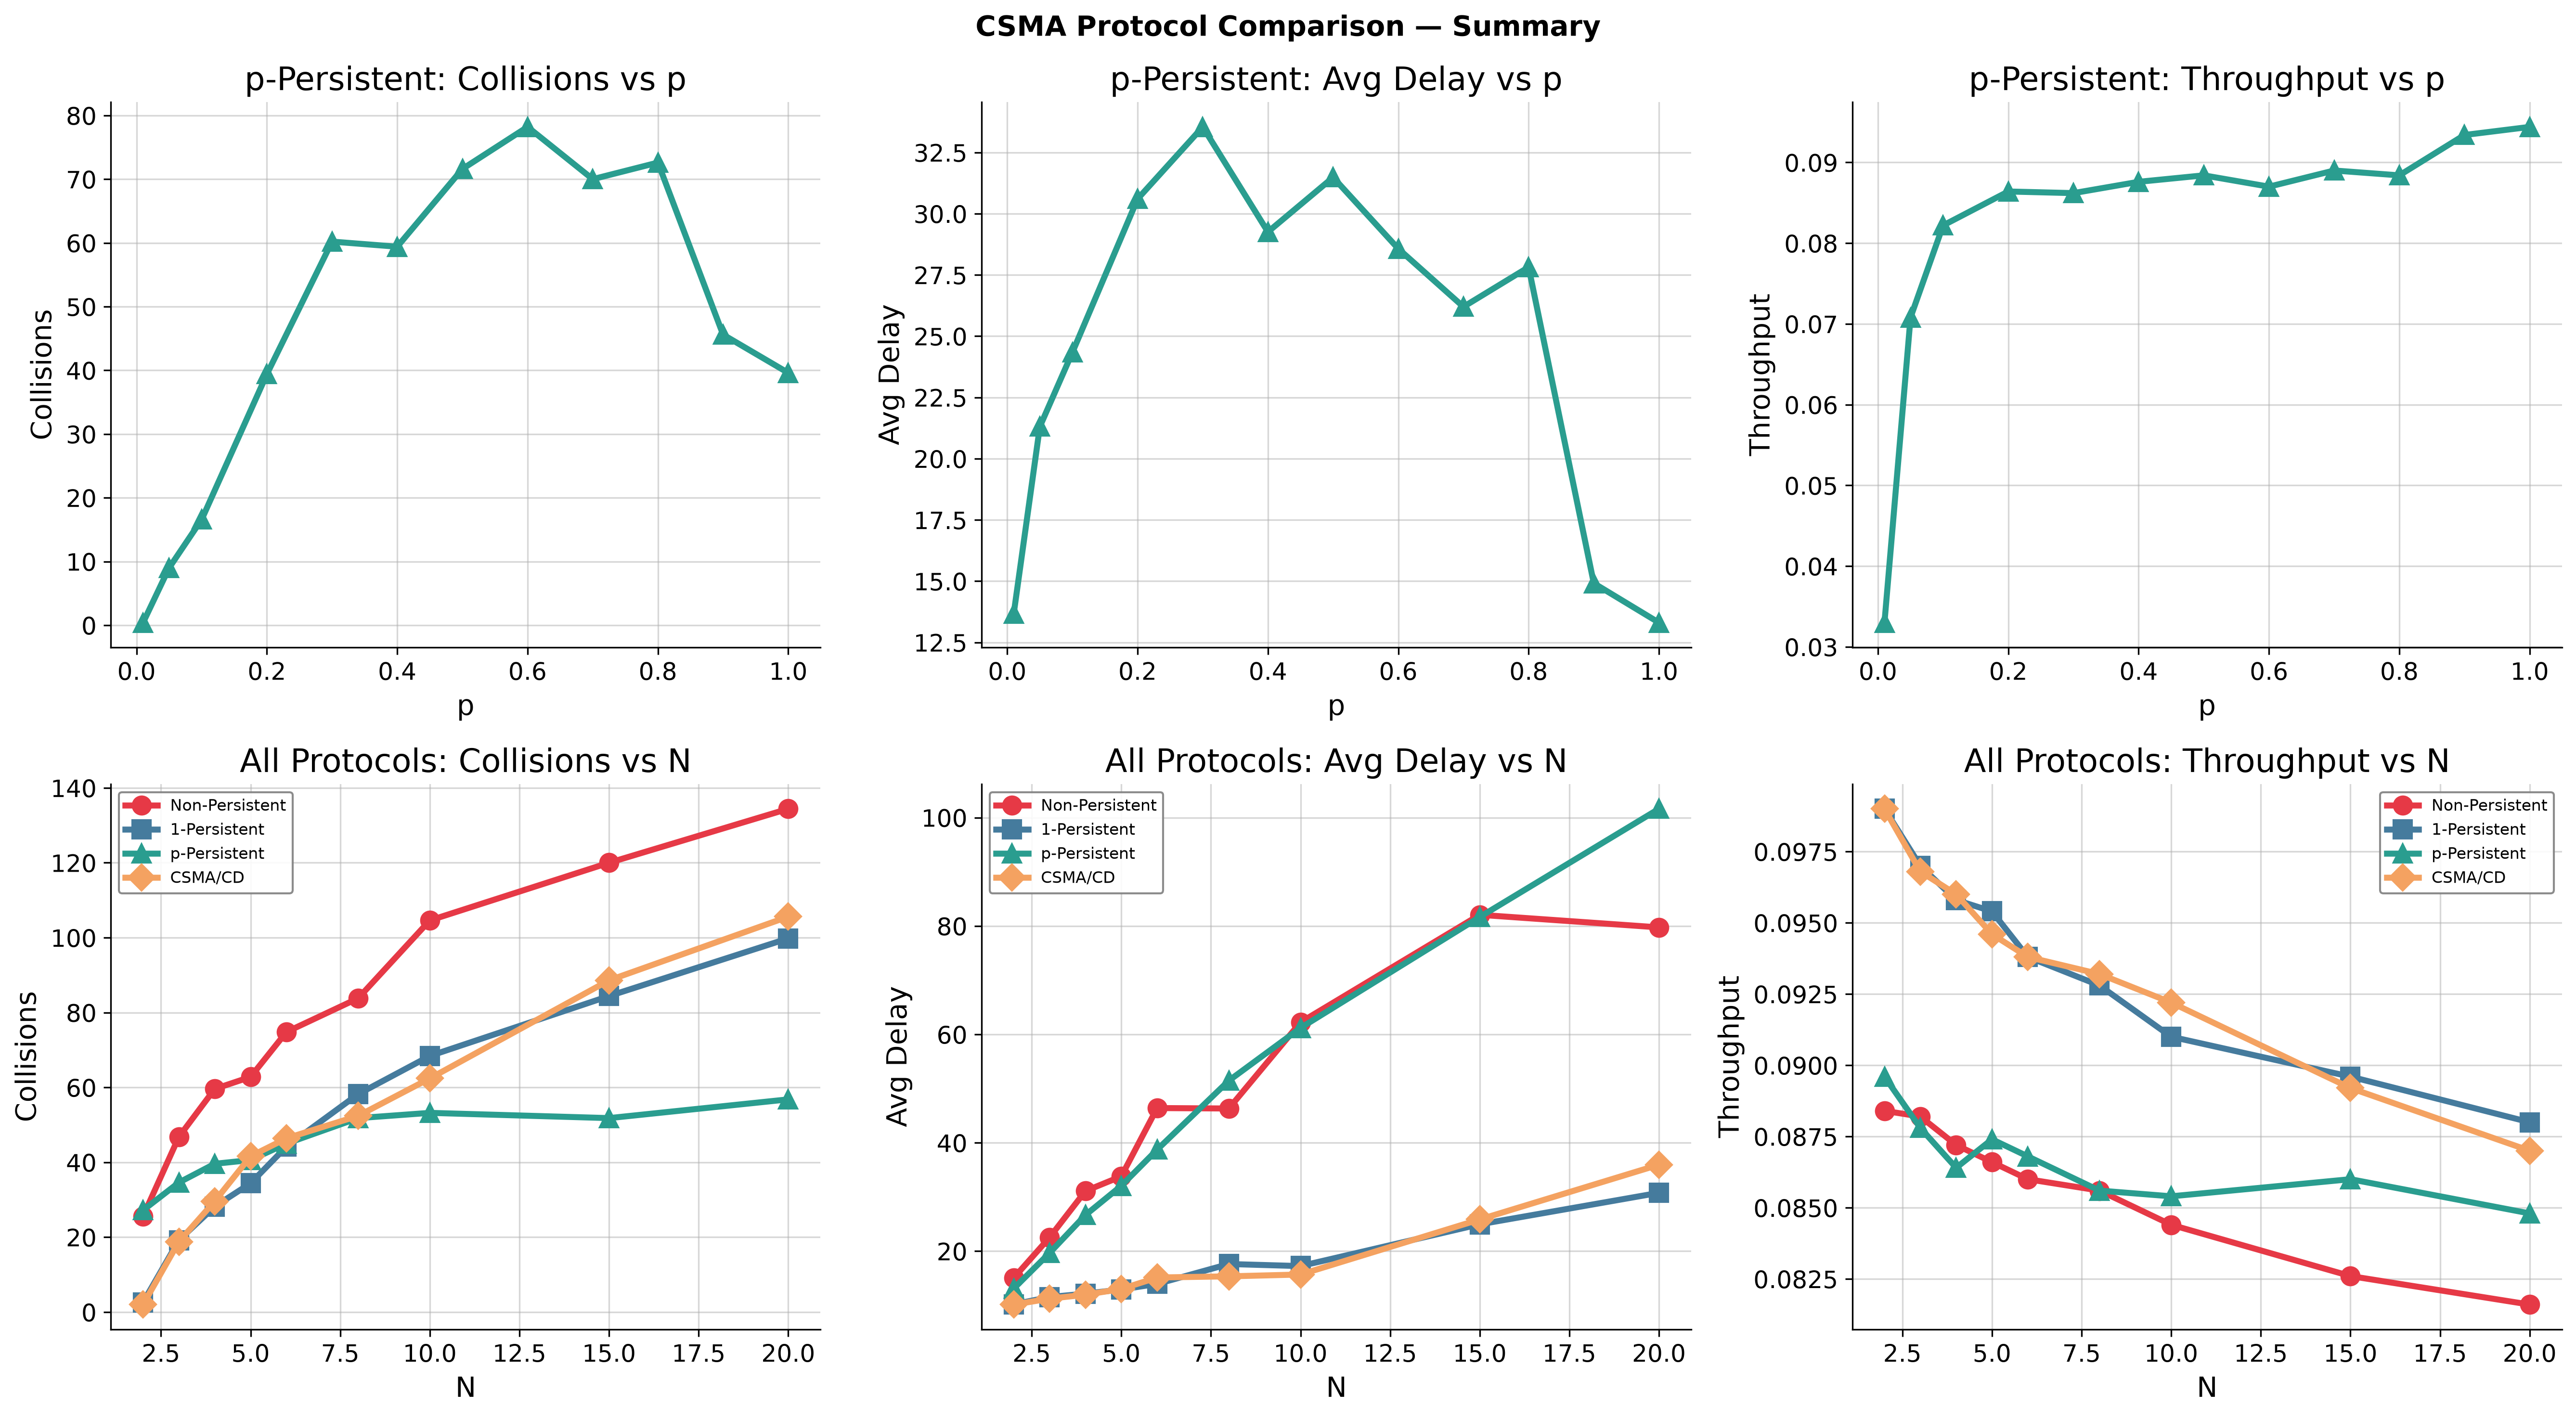
\includegraphics[width=0.7\textwidth]{plots/fig7_combined_summary.png}
    \caption{Combined Simulation Summary}
\end{figure}

As shown in the figures, CSMA/CD maintains robust throughput under high load compared to 1-Persistent CSMA, which collapses under high contention due to the vulnerability window.

\section{Analysis}

\begin{itemize}
    \item \textbf{Correctness:} The simulation accurately matches theoretical ALOHA and CSMA performance envelopes. Throughput follows the classic G/G/1 queuing model saturation curve.
    \item \textbf{Results Discussion:} p-Persistent ($p=0.1$) scales surprisingly well under high node density ($N > 15$) because the deliberate deferral breaks synchronization among waiting nodes. 1-Persistent behaves best at low loads where latency is prioritized over collision avoidance. CSMA/CD is the overall most robust, as aborting early prevents long frames from unnecessarily occupying the channel during a collision.
    \item \textbf{Known Bugs \& Fixes:} Initially, the live dashboard reported a 0\% collision rate. This was due to the \texttt{check\_collision} abort step clearing the active transmitter list \textit{before} the slot state logger was called. By refactoring the state logger to rely on a decoupled \texttt{busy\_until} variable, accurate metric tracking was achieved.
\end{itemize}

\section{Comments}

This lab assignment provided exceptional insight into the hidden complexities of network medium access control. 
\begin{itemize}
    \item \textbf{Difficulty:} The assignment was moderately difficult. Building the independent \texttt{Station} queues was straightforward, but managing the synchronized, discrete-event state of the \texttt{Channel} (handling propagation delays and simultaneous multi-station TX attempts) required precise order-of-operations logic in the simulation loop.
    \item \textbf{Learning Outcomes:} I gained hands-on experience with discrete-event simulation, concurrency modeling, and Python application development (including a \texttt{Rich} terminal dashboard).
    \item \textbf{Improvements:} An interesting extension would be incorporating hidden-terminal problem topologies (modeling distance graphs rather than a single unified broadcast bus) to evaluate CSMA/CA (RTS/CTS).
\end{itemize}

\end{document}
